\documentclass[usepdftitle=false]{beamer}

\usepackage[T1]{fontenc}

\usepackage[utf8x]{inputenc}
\usepackage{default}
\usepackage{lmodern}
\usepackage{booktabs}

\usepackage{ragged2e} % Kommando\justifying ermöglicht  Blocksatz in Präsentationen

\mode<presentation>
 {\usecolortheme{seahorse,rose}
 \useinnertheme[shadow]{rounded}
%  \useoutertheme[hideothersubsections,right,width=4em,frame number]{sidebar}
%  \useoutertheme{infolines}
%\useoutertheme{split}
\useoutertheme[subsection=false,footline=authortitle]{miniframes}
\setbeamercovered{transparent}
}

%seitenzahl in linker ecke
\addtobeamertemplate{navigation symbols}{{\usebeamercolor{section
in toc}\footnotesize
\insertframenumber/\inserttotalframenumber}\hspace{48em}}{}
\usepackage{setspace} %mit spacing-Umgebung Zeilenabstand regeln



%%Sprachunterstuetzung
%Englische Silbentrennung, etc.
\usepackage[spanish]{babel}
%Mehrsprachige Literaturliste
\usepackage{babelbib}
%%Graphiken und Farbe
%Graphiken
\usepackage{graphicx} 
%von beamer.cls geladen
%Farbe
\usepackage{color,pgf}
%von beamer.cls geladen
%PDF-Seiten einbinden
\usepackage{pdfpages}
\usepackage{subscript}
\newcommand{\sub}[1]{\textsubscript{#1}}
\newcommand{\Sup}[1]{\textsuperscript{#1}}
\newcommand{\COO}{CO\textsubscript{2}}
\newcommand{\masl}{m~a.s.l.}
\newcommand{\gc}{$^{\circ}$C}
\newcommand{\tilt}{$\sim$}
\newcommand{\blue}[1]{{\color{blue!50!black}#1}}
\newcommand{\Blue}[1]{{\color{blue!50!black}\textbf{#1}}}
\newcommand{\eg}{e.\,g.}
\newcommand{\Eg}{E.\,g.}

% new environment for slides with changes margins
\newenvironment{changemargin}[2]{%
\begin{list}{}{%
\setlength{\topsep}{0pt}%
\setlength{\leftmargin}{#1}%
\setlength{\rightmargin}{#2}%
\setlength{\listparindent}{\parindent}%
\setlength{\itemindent}{\parindent}%
\setlength{\parsep}{\parskip}%
}%
\item[]}{\end{list}}





\hypersetup{
pdfauthor={Roman Link},
pdftitle={Introducción XylEm Plus + bomba de Scholander},
}

%Titelseite
\title{Introducción al uso del XylEm Plus y de la bomba de Scholander}
\subtitle{\normalfont Curso de laboratorio \textit{Mediciones de hidráulica de plantas con el XylEm Plus y la bomba de Scholander}}
\author[R. Link]{Roman Link}
\date{27 de noviembre de 2017}
\institute[University of Göttingen]{
Department of Plant Ecology and Ecosystem Research\\ Georg August University of Göttingen}
%\titlegraphic{ \vspace*{2em}
%
\includegraphics[width=0.7\textwidth]{logouni.png}}%oder was sch\"oneres

\logo{
\includegraphics[width=20em]{logounisolow.png}}

\usepackage{amsmath,amsfonts,amssymb,pgf}
 \usepackage { eulervm }

%\usepackage[round]{natbib}
%\def\newblock{} % hilft gegen absurde fehler mit natbib

\newcommand{\rar}{$\rightarrow$}
\newcommand{\lar}{$\leftarrow$}
\newcommand{\Rar}{$\Rightarrow$}
\newcommand{\Lar}{$\Leftarrow$}
\newcommand{\quelle}[1]{\baselineskip8pt{\tiny \color{gray} #1}}

\newcommand{\tw}{\textwidth}
\newcommand{\ddx}[2]{\frac{\mathrm{d}}{\mathrm{d}#2}#1 }
\newcommand{\ddxx}[2]{\frac{\mathrm{d^2}}{\mathrm{d}#2^2}#1}



\newcommand{\code}[1]{{\footnotesize \color{blue}
\texttt{#1}}\normalsize\color{black}}


% \input{cc_beamer}
\setbeamerfont{section in toc}{size=\normalsize,series=\bfseries}
\setbeamerfont{title}{series=\bfseries}
\setbeamerfont{frametitle}{size=\Large,series=\bfseries}

\begin{document}


%%%%%%%%%%%%%%%%%		Title Page			%%%%%%%%%%%%%%%%%%%%%%
\begin{frame}
\titlepage
\end{frame}


%%%%%%%%%%%%%%%%%%%%%%%%%%%%%%%%%%%%%%%%%%%%%%%%%%%%%%%%%%%%%%%%%%%%
\section{XylEm Plus}
%%%%%%%%%%%%%%%%%%%%%%%%%%%%%%%%%%%%%%%%%%%%%%%%%%%%%%%%%%%%%%%%%%%%
\begin{frame}
	\frametitle{El XylEm Plus}
	\centering{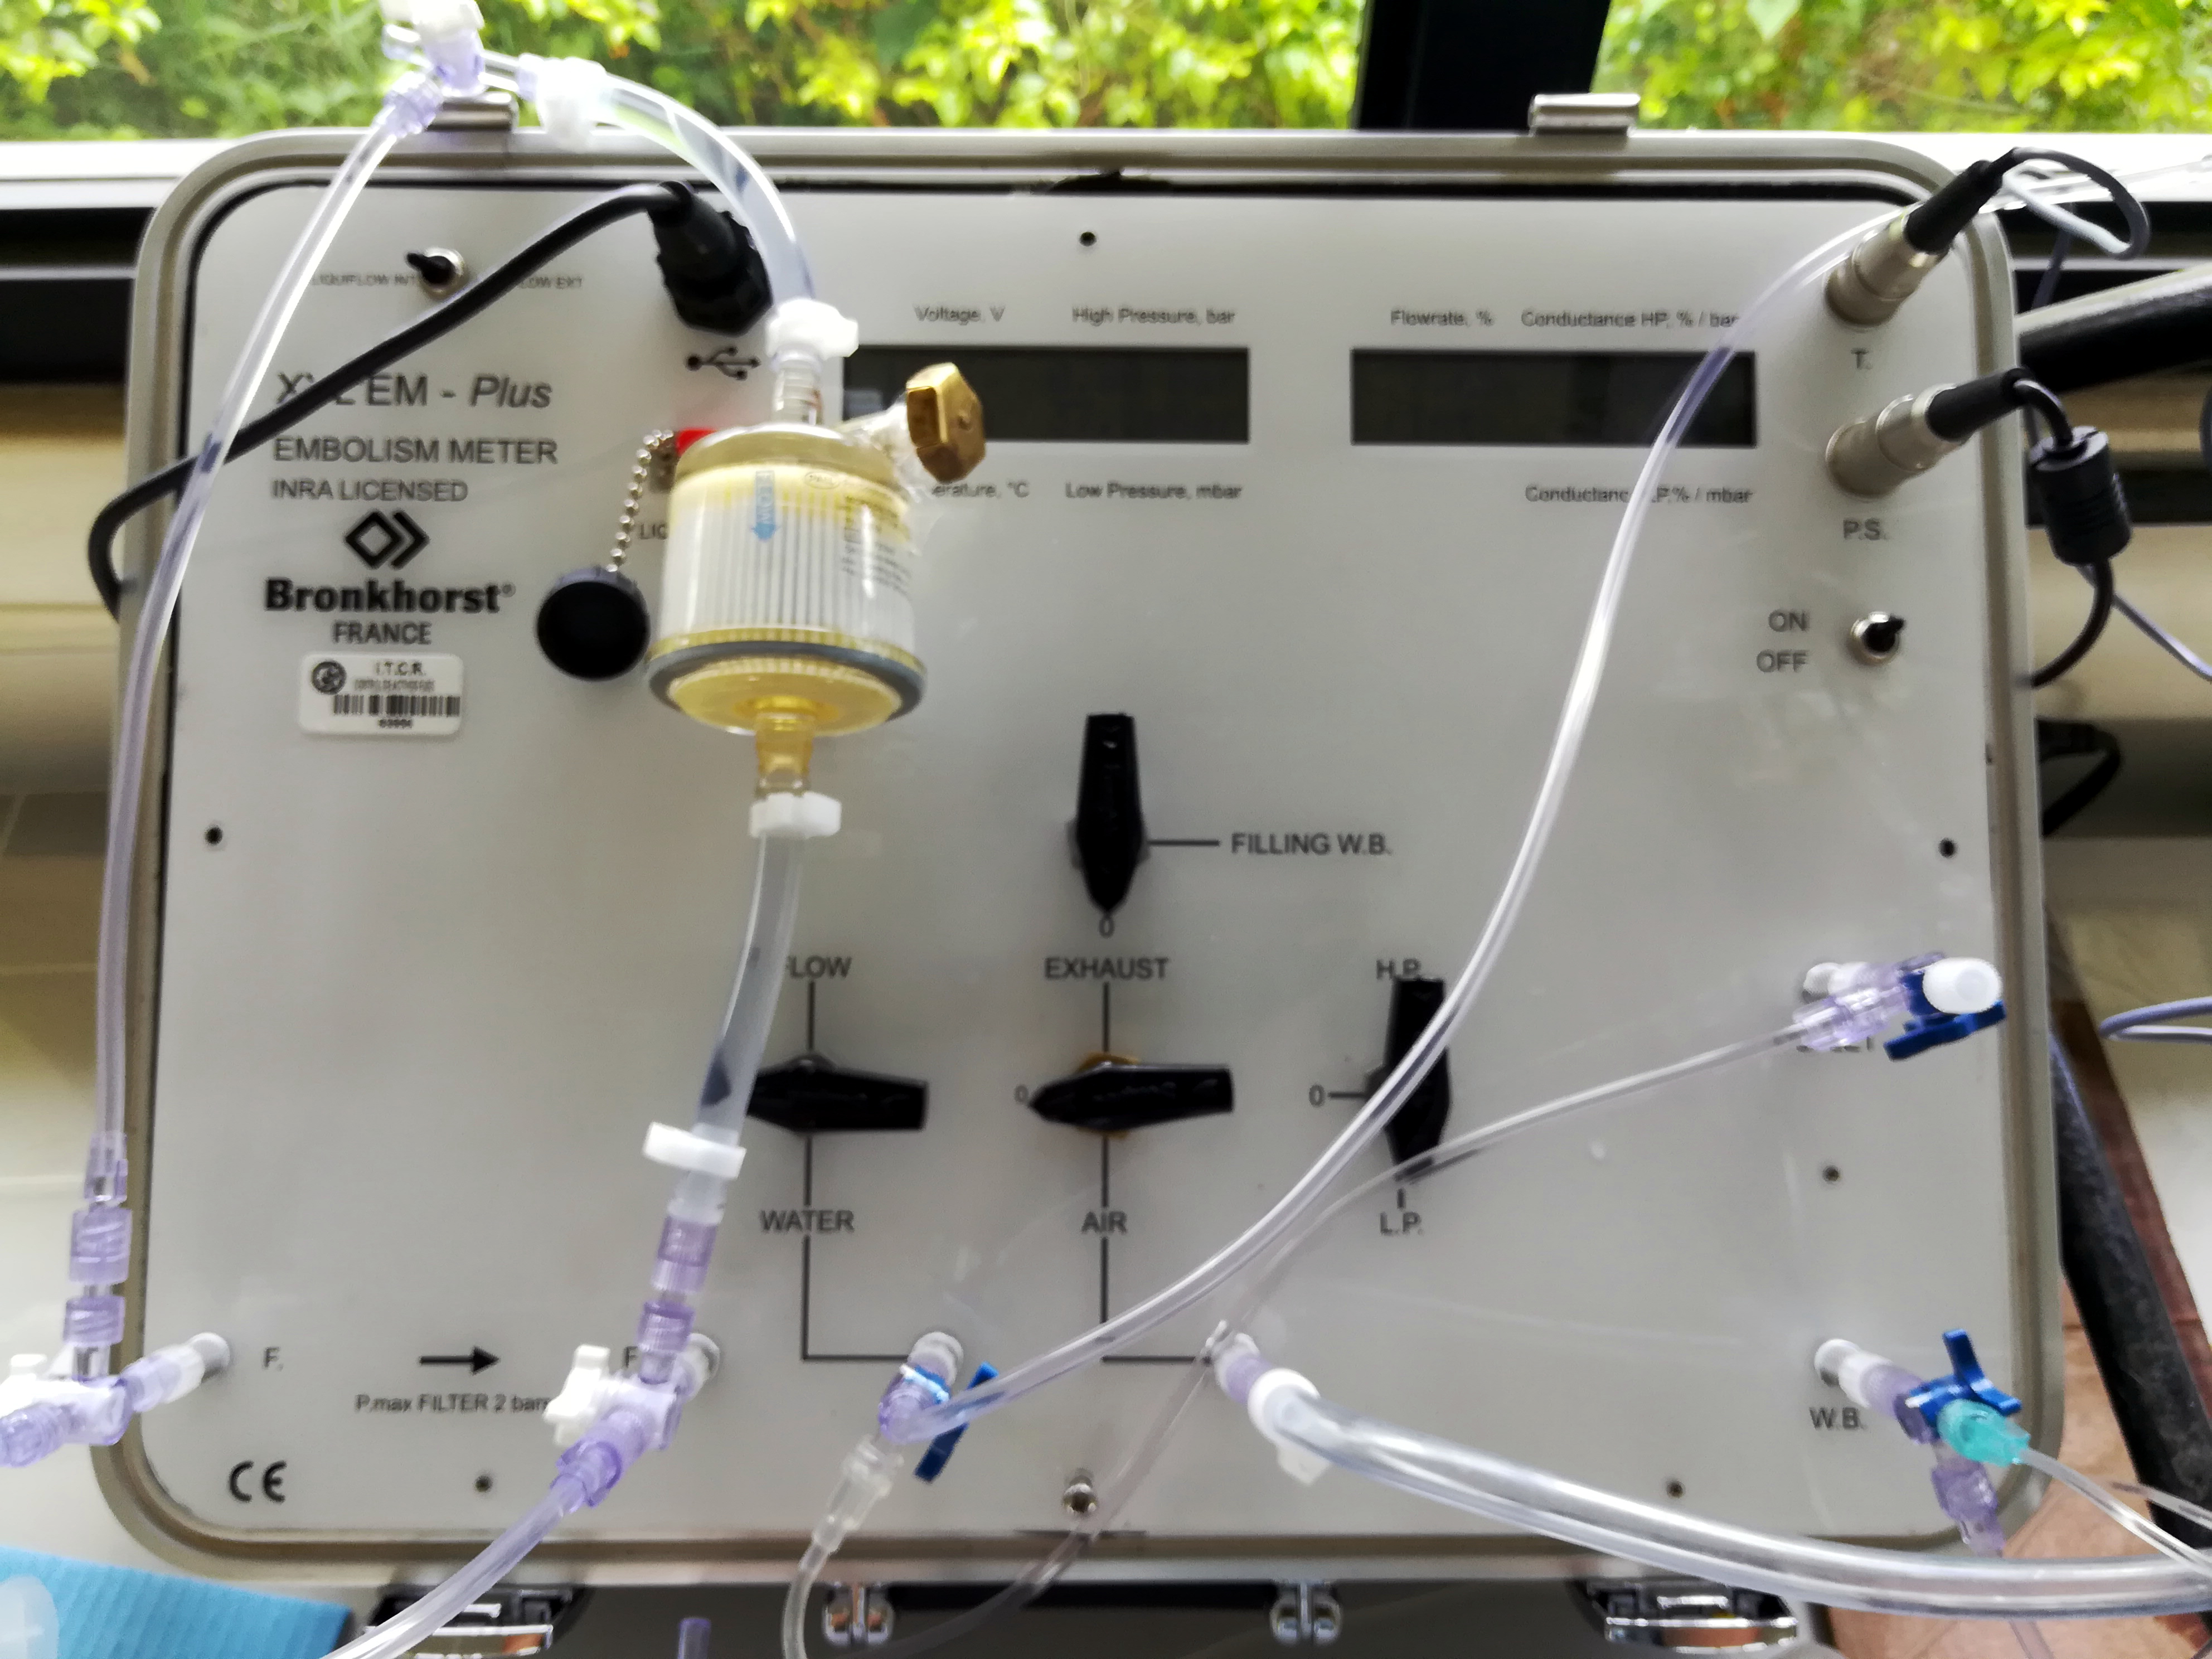
\includegraphics[width = 0.7\tw]{pictures/xylem.jpg}} 
   \only<1>{
   	\begin{itemize}
   	\item Sistema integrado para \alert{mediciones de conductividad} de muestras de madera o tallos de plantas herbaceas
   	\item Mide tasa de flujo (g/h) y presión de agua (mbar) 
   \end{itemize}
   	}
   \only<2>{
   	\begin{itemize}
   		\item \alert{XylEm}: Prototipo desarrollado en 2000-2002 (Cochard et al. 2000, Cochard et al. 2002, Cochard 2002)
   		\item Cambio del diseño en 2012: \alert{XylEm Plus} (Bronkhorst, Francia)
   	\end{itemize}
   }			
\end{frame}

\begin{frame}
	\frametitle{Funcionamiento del XylEm Plus}
	\begin{minipage}{0.5\tw}
		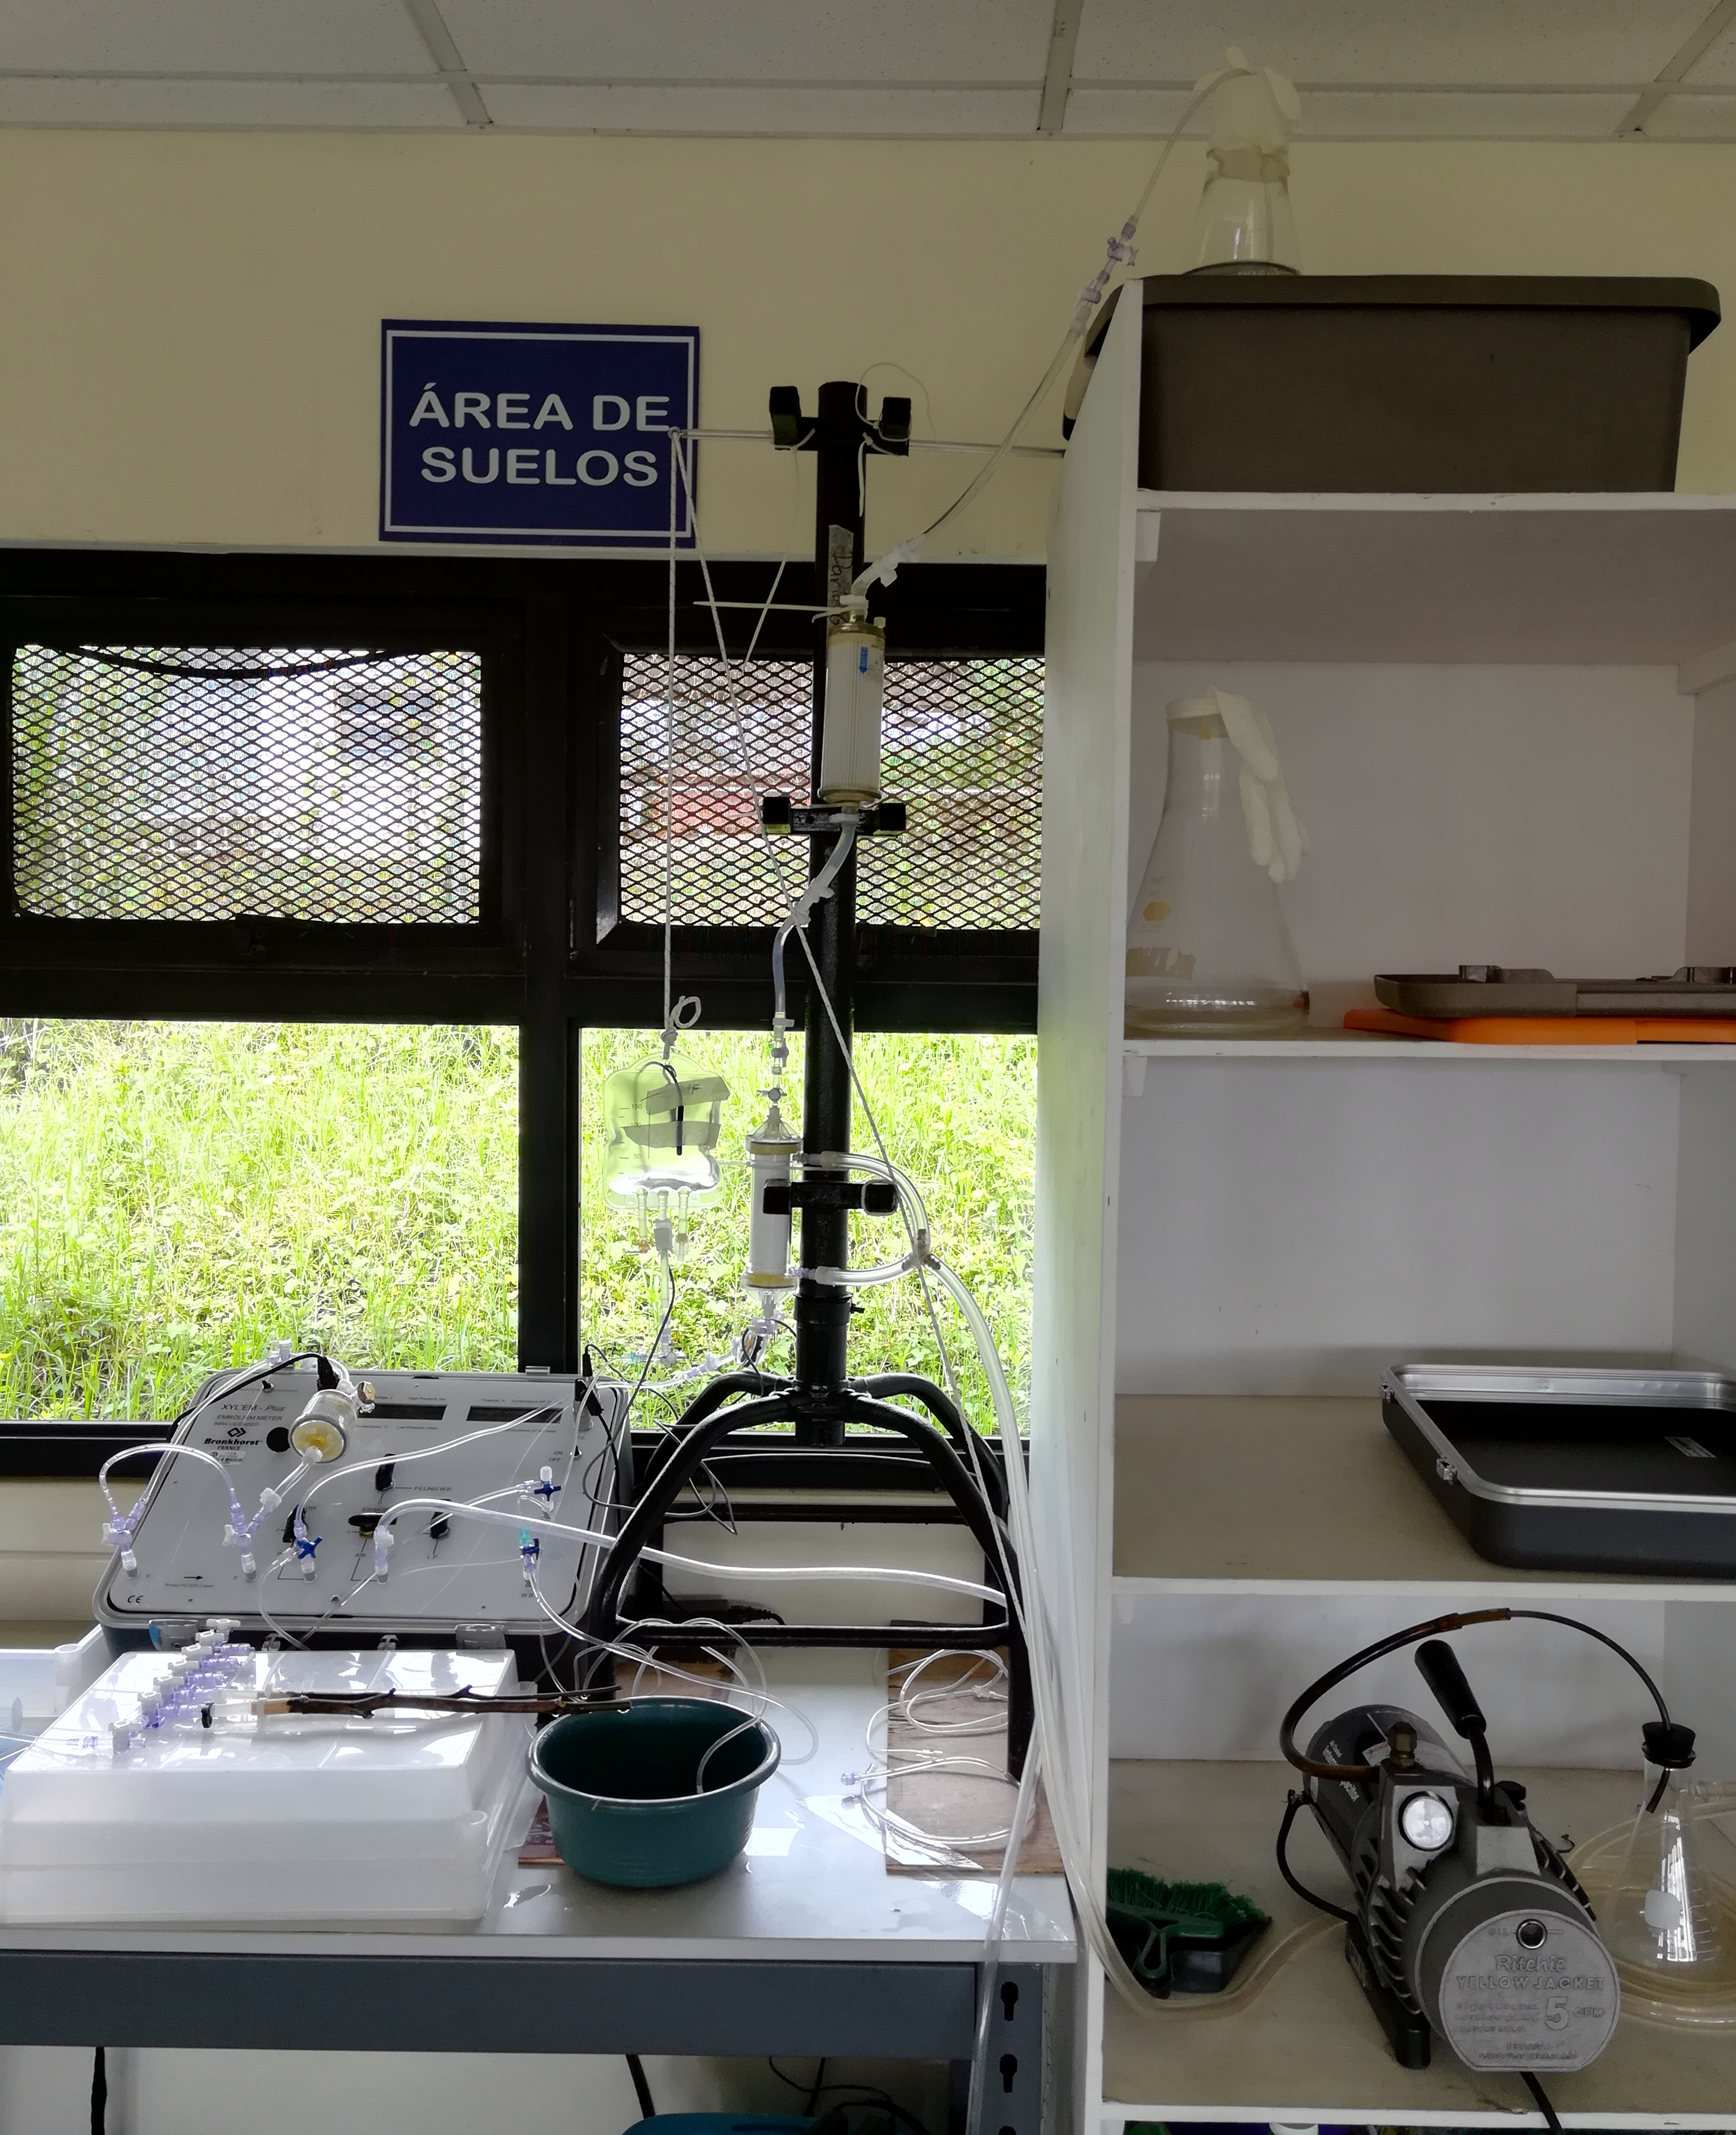
\includegraphics[width =\tw]{pictures/xylem_completo.jpg} 
	\end{minipage}
	\begin{minipage}{.48\tw}
		\begin{itemize}
			\item Basado en el principio del \textit{\alert{aparato de Sperry}} (Sperry et al., 1988)
			\item Presión de agua generada por gravedad
			\item Muestras conectado con sistema de Luer Lok
		\end{itemize}		
	\end{minipage}
\end{frame}

\begin{frame}	
	\frametitle{Funcionamiento del XylEm Plus}
		\begin{minipage}{0.5\tw}
			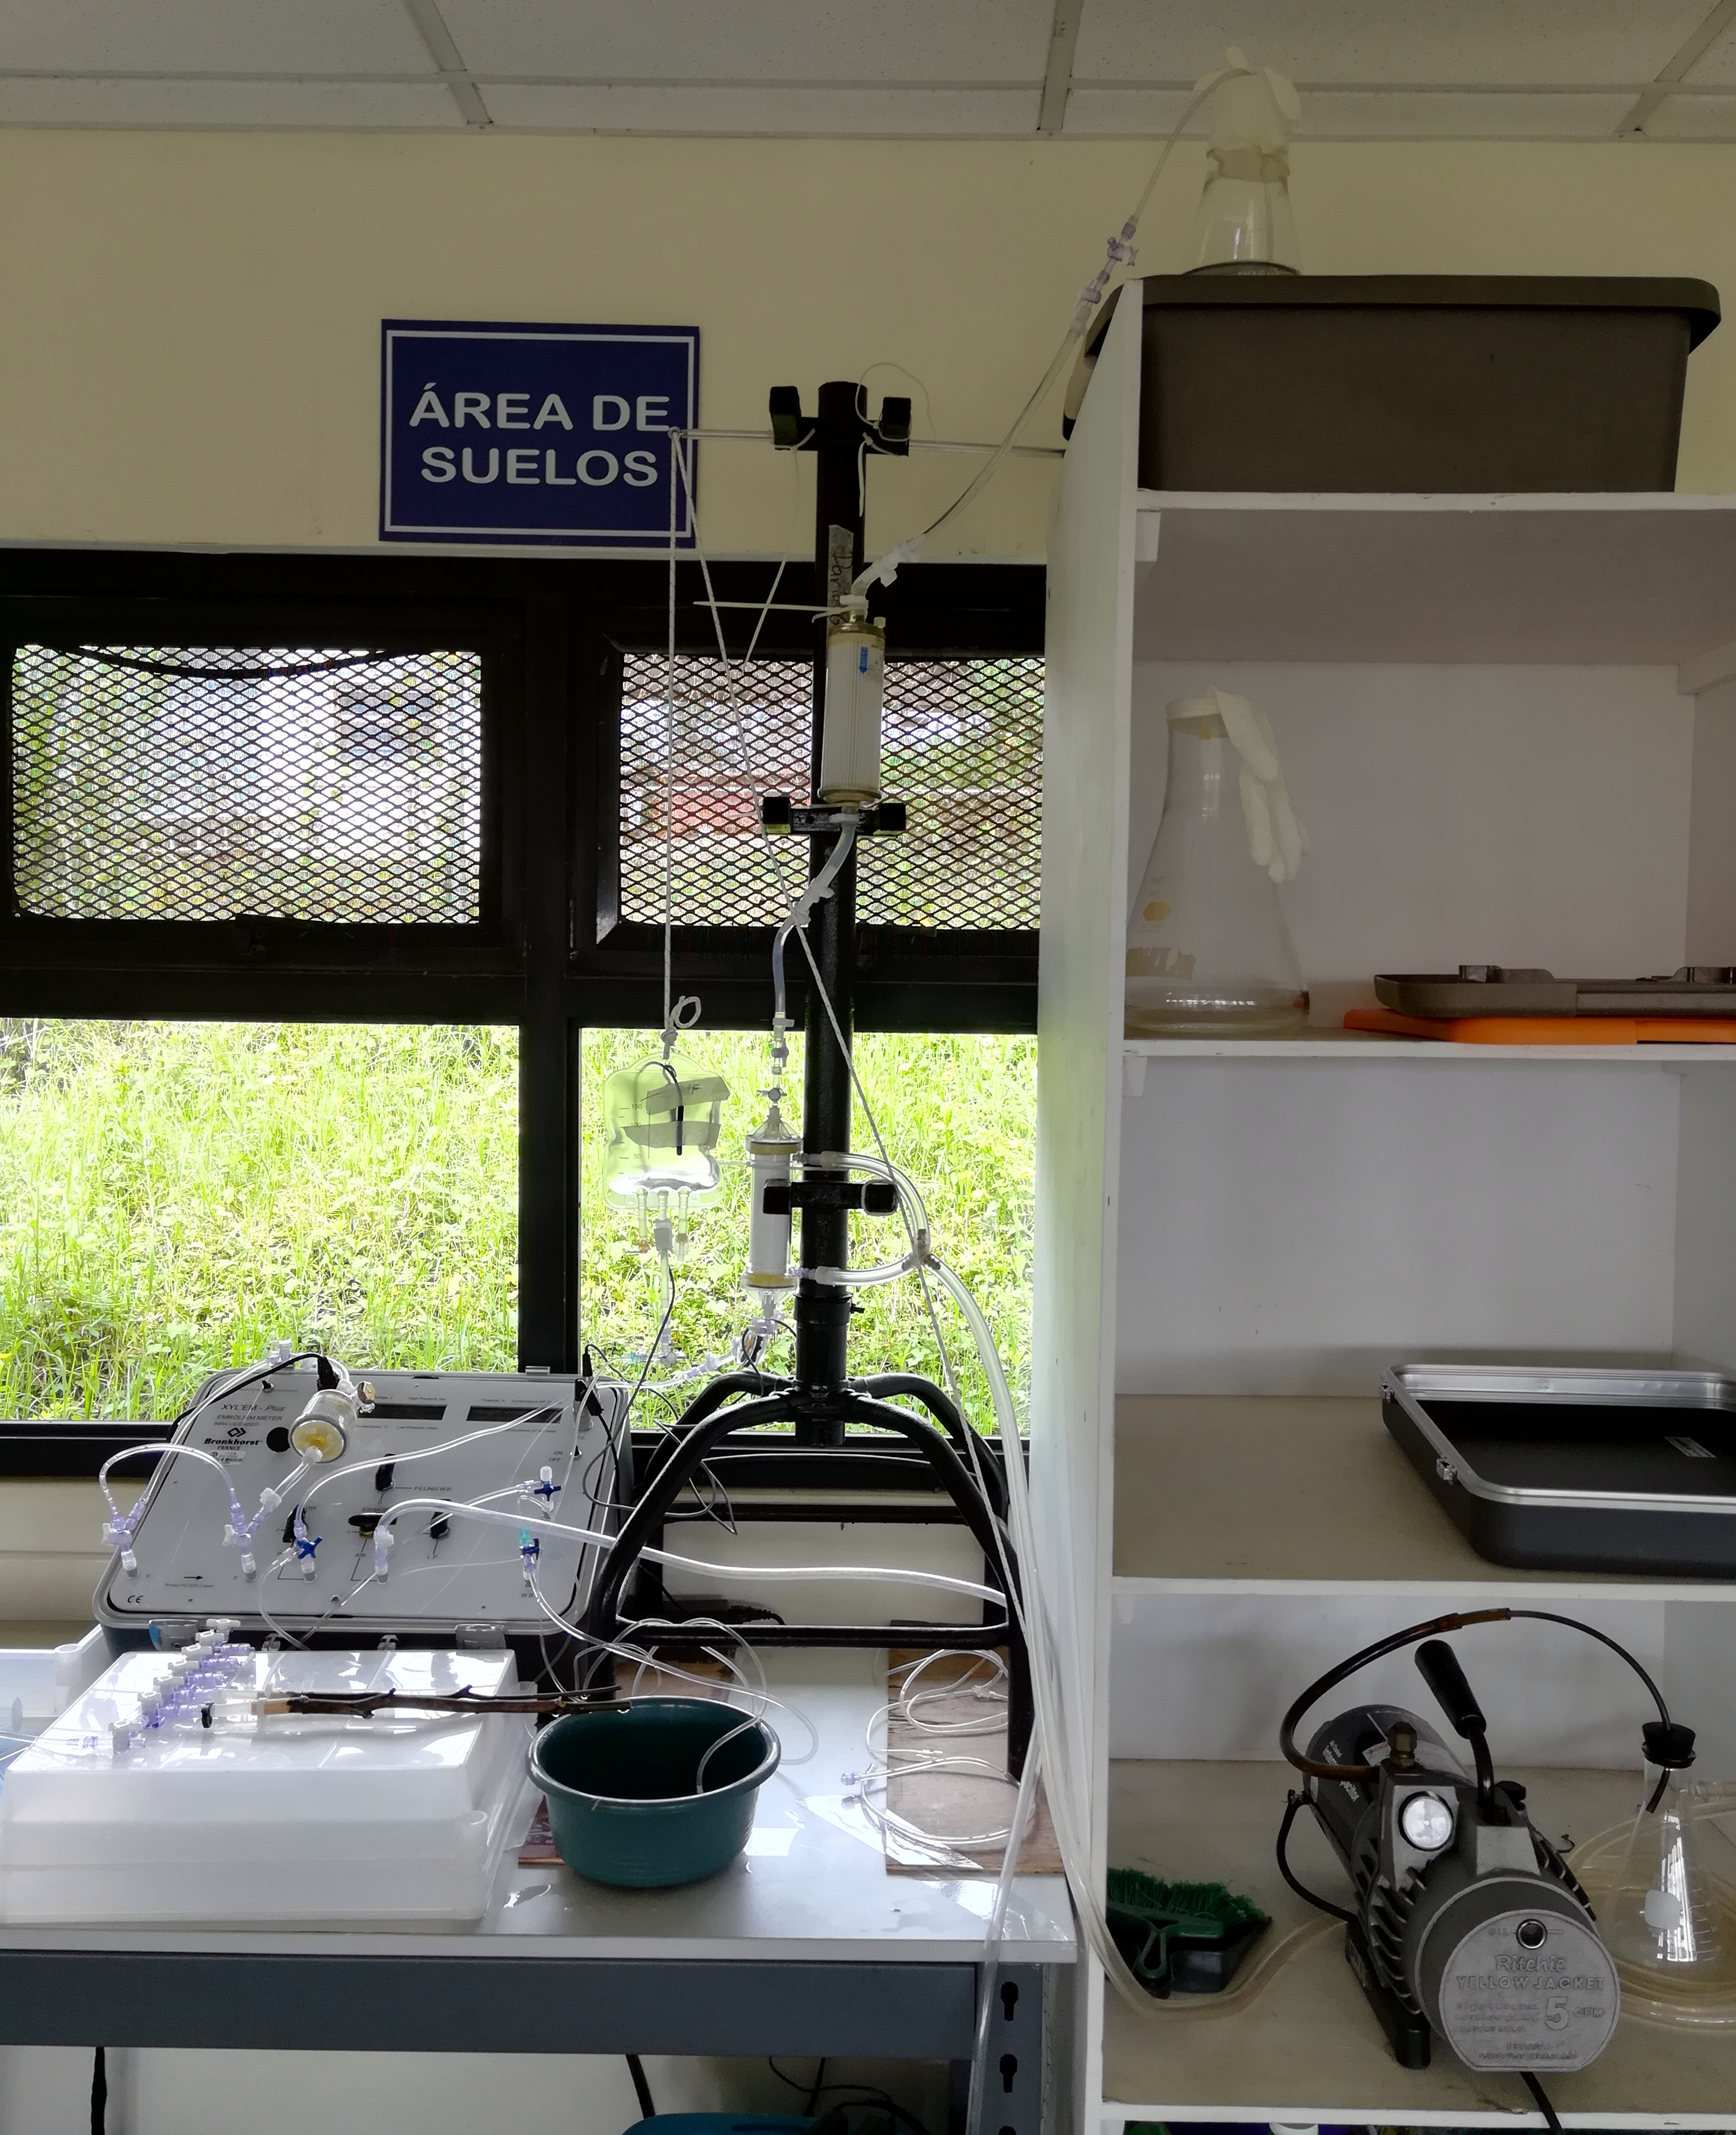
\includegraphics[width =\tw]{pictures/xylem_completo.jpg} 
		\end{minipage}
		\begin{minipage}{.48\tw}
        	\begin{itemize}
				\item \alert{Solución de medición}: Agua ultrapura (grado I) desgasificada con 10 mmol KCl, 1 mmol CaCl$_2$
				\item Antes de pasar por las muestras, pasa por dos filtros de partículos (5 µm) y un filtro de vacío
        	\end{itemize}		
		\end{minipage}	
\end{frame}

\begin{frame}	
	\frametitle{Diagráma de flujo del XylEm Plus}	
    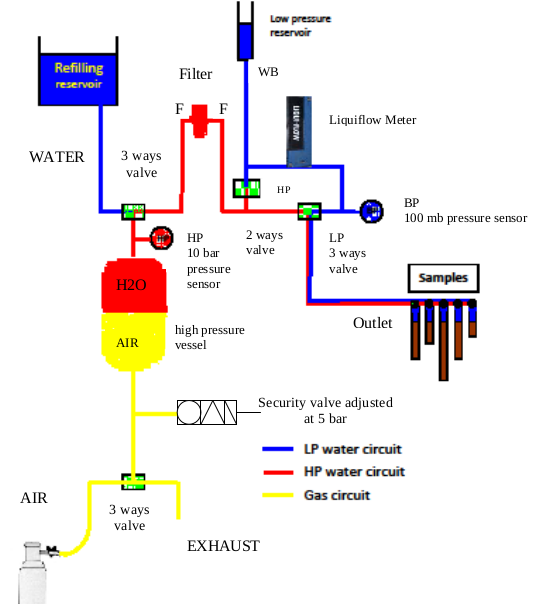
\includegraphics[width =0.68\tw]{pictures/xylem_fluid_diagram.png} 
    	
\vspace{-2.5em}    	
\centering{\quelle{\textbf{Ilustración:} Hervé Cochard, 2013.}}
\end{frame}



\begin{frame}	
	\frametitle{Preparación de muestras}
	\begin{minipage}{.68\tw}
		\begin{itemize}
			\item Cortar con cuchilla muy afilada
			\item Diámetro: idealmente 5-10 (15) mm
			\item Longitud: idealmente mayor a la \alert<3>{longitud máxima de vasos}
		\end{itemize}	    	
	\end{minipage}
	\begin{minipage}{0.3\tw}
		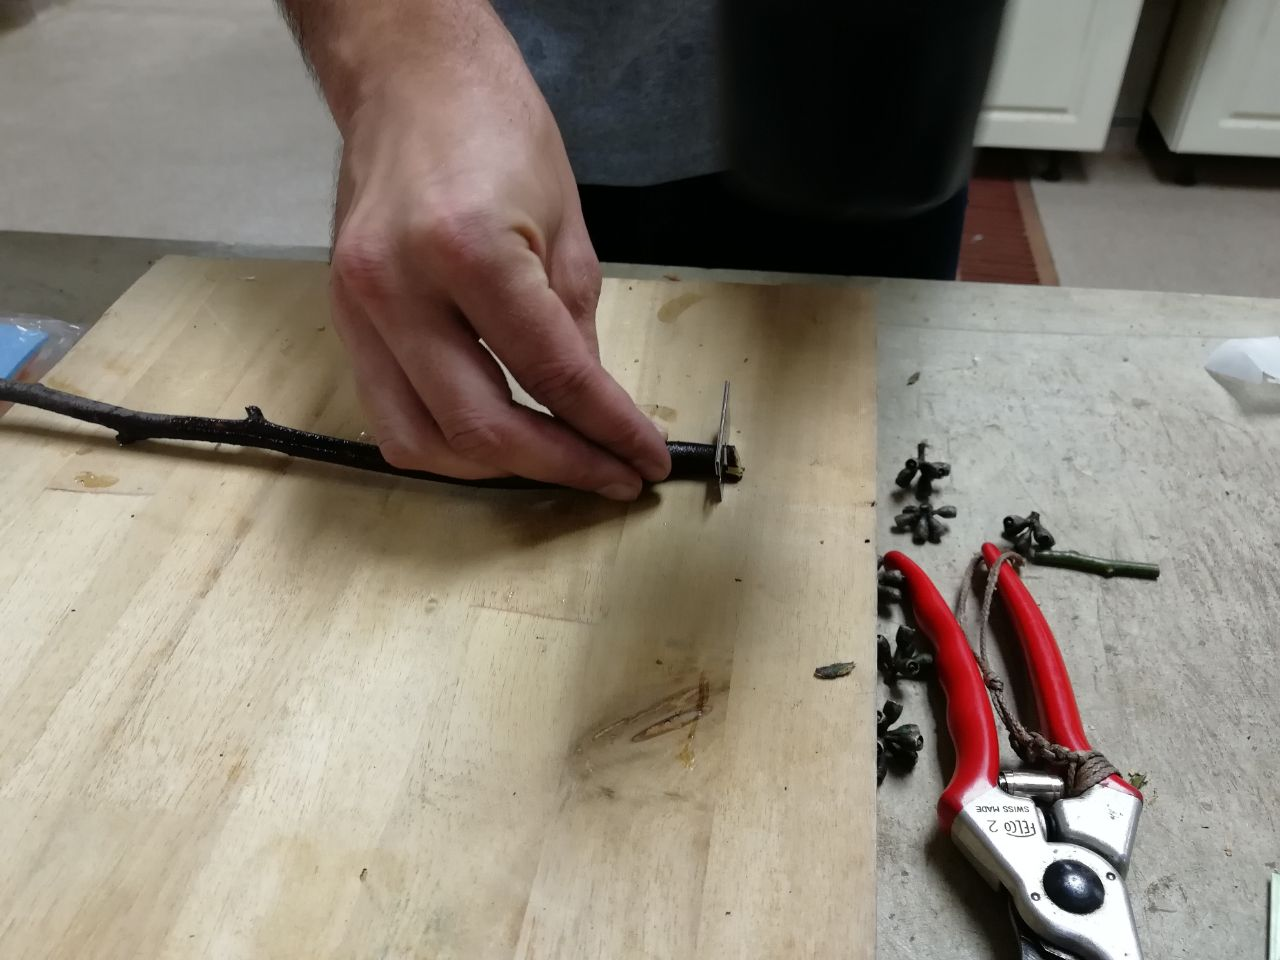
\includegraphics[width =\tw]{pictures/muestras3.jpg}
		
		\only<1>{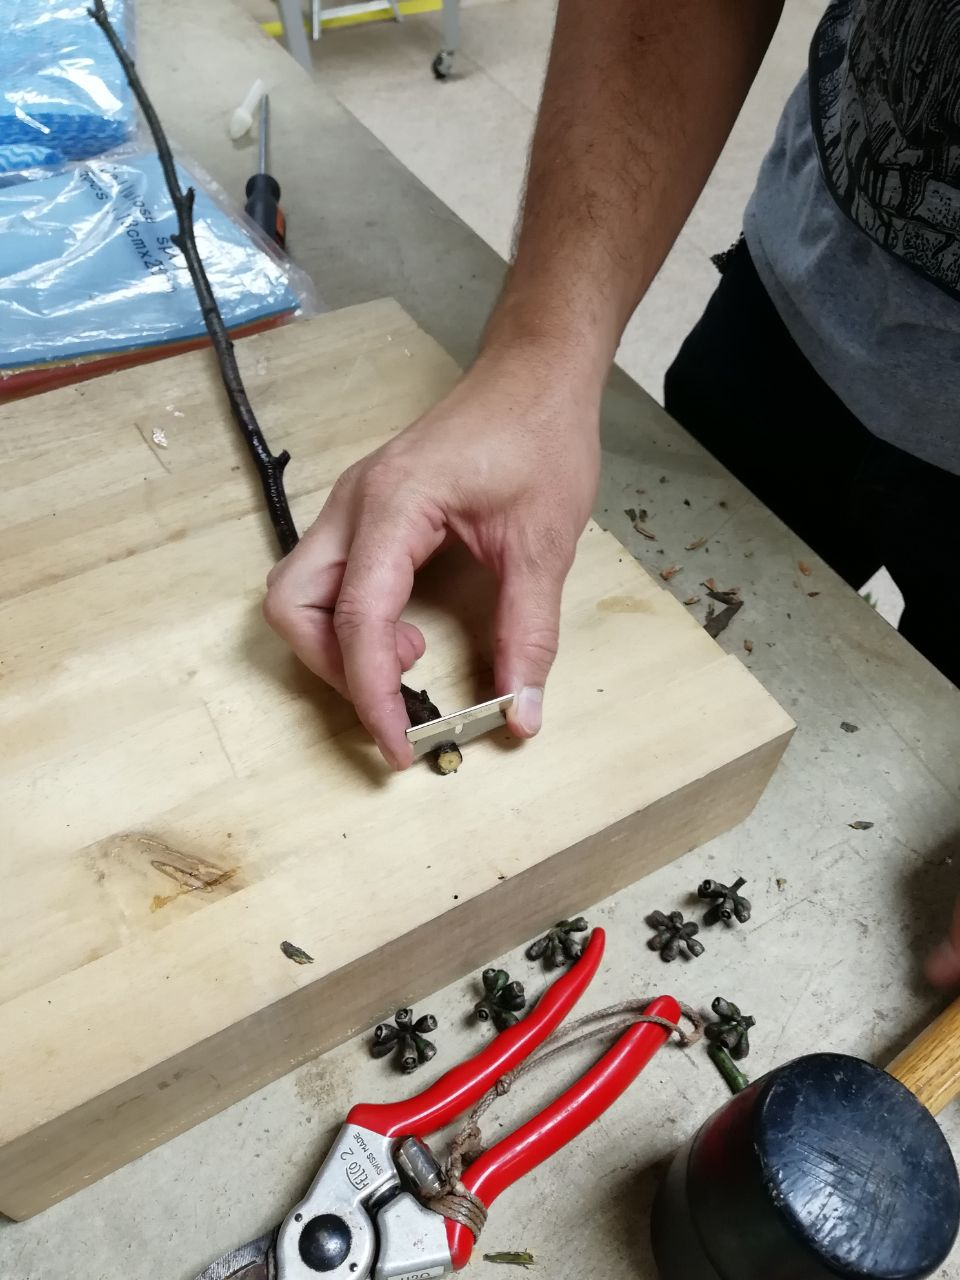
\includegraphics[width =\tw]{pictures/muestras2.jpg}}
		
		\only<2-3>{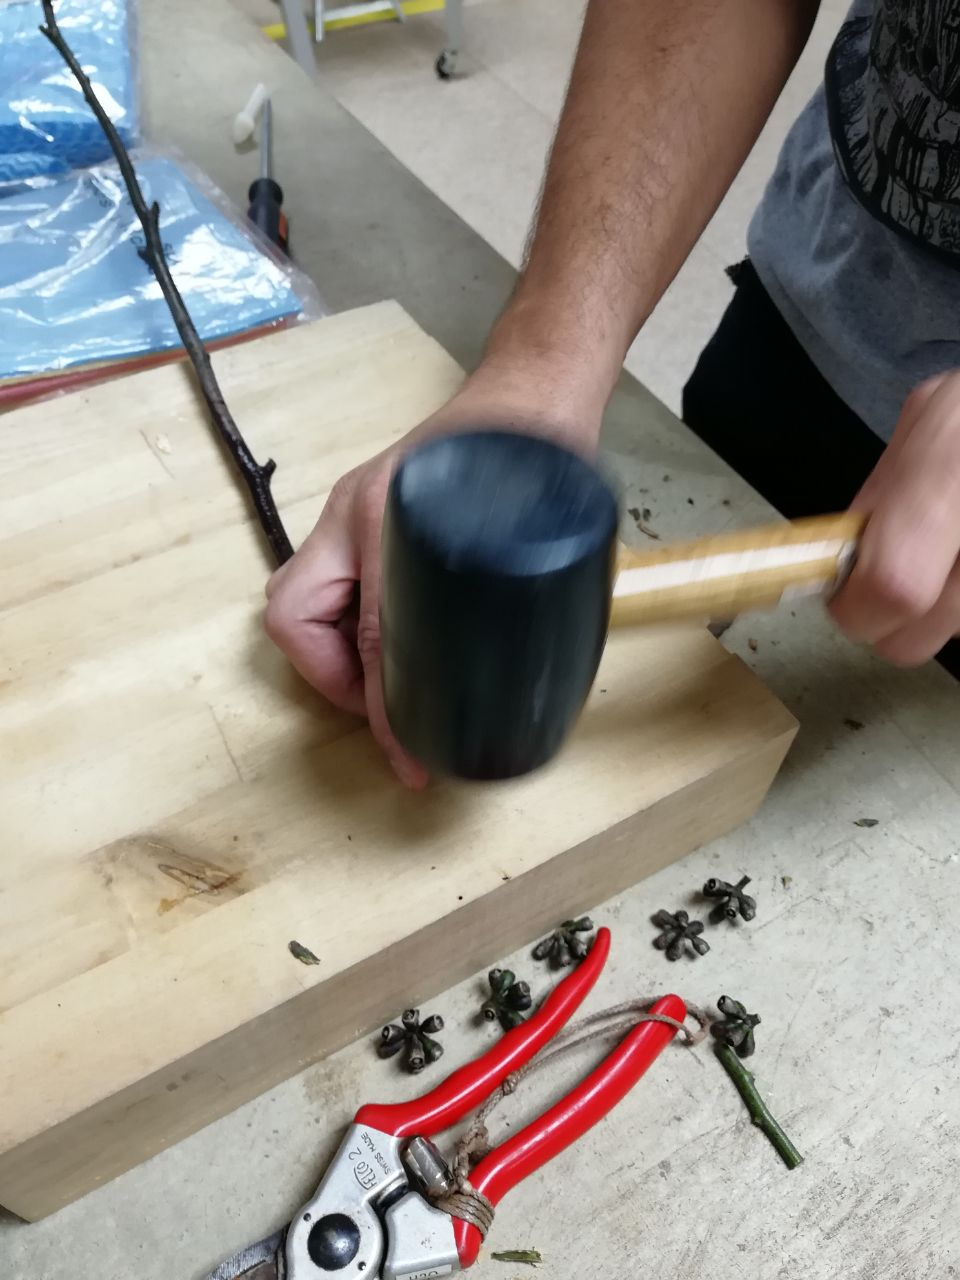
\includegraphics[width =\tw]{pictures/muestras1.jpg}}	  
	\end{minipage}			
\end{frame}

\begin{frame}	
	\frametitle{Longitud máxima de vasos}
	\begin{minipage}{.5\tw}
		\textbf{Protocolo de medición:}
		\begin{itemize}
			\item<1- |alert@1> Conectar el lado acropeto de la muestra con tubo de látex
			\item<2- |alert@2> Generar presión de ~1 bar con jeringa
			\item<3- |alert@3> Cortar trozos de 1-5 cm varias veces hasta que salgan burbujas del lado basípeto (el aire solo puede pasar por vasos abiertos en ambos lados)				
		\end{itemize}	    
		\visible<4>{\textbf{\alert{¡Solo un estimado muy crudo!}}}	
	\end{minipage}
	\begin{minipage}{0.48\tw}		
		\only<1>{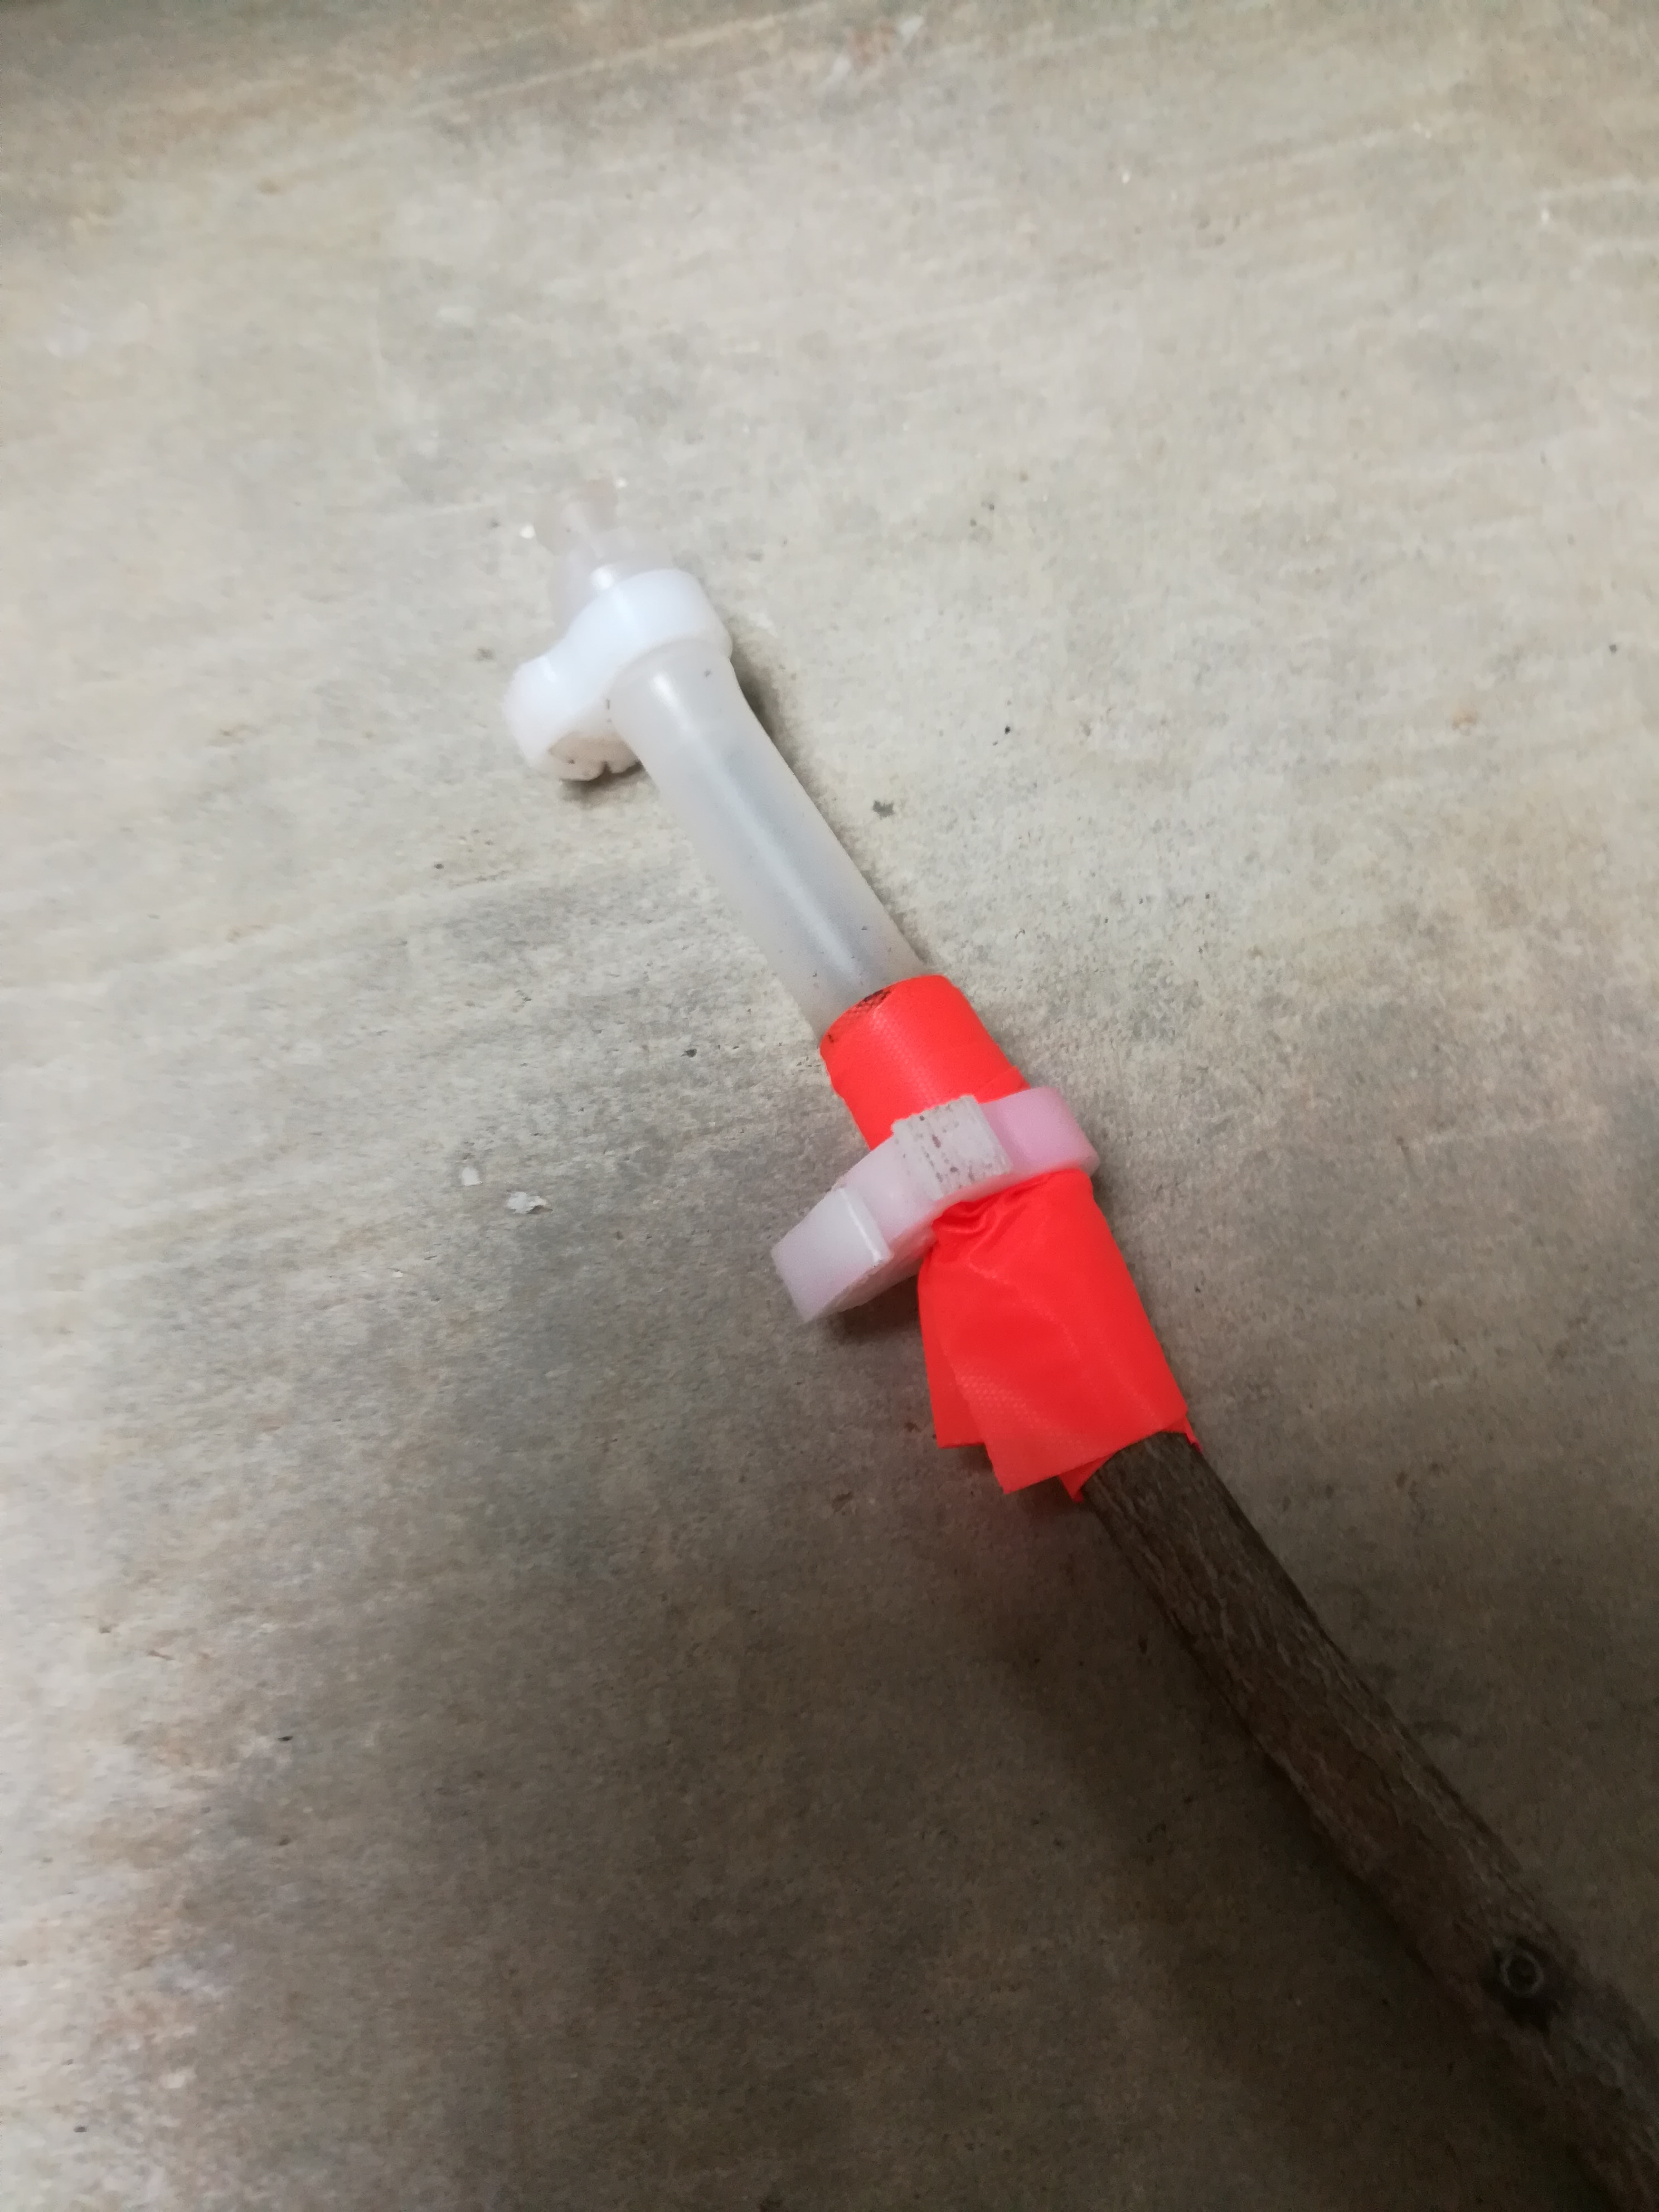
\includegraphics[width =\tw]{pictures/VL1.jpg}}
		
		\only<2>{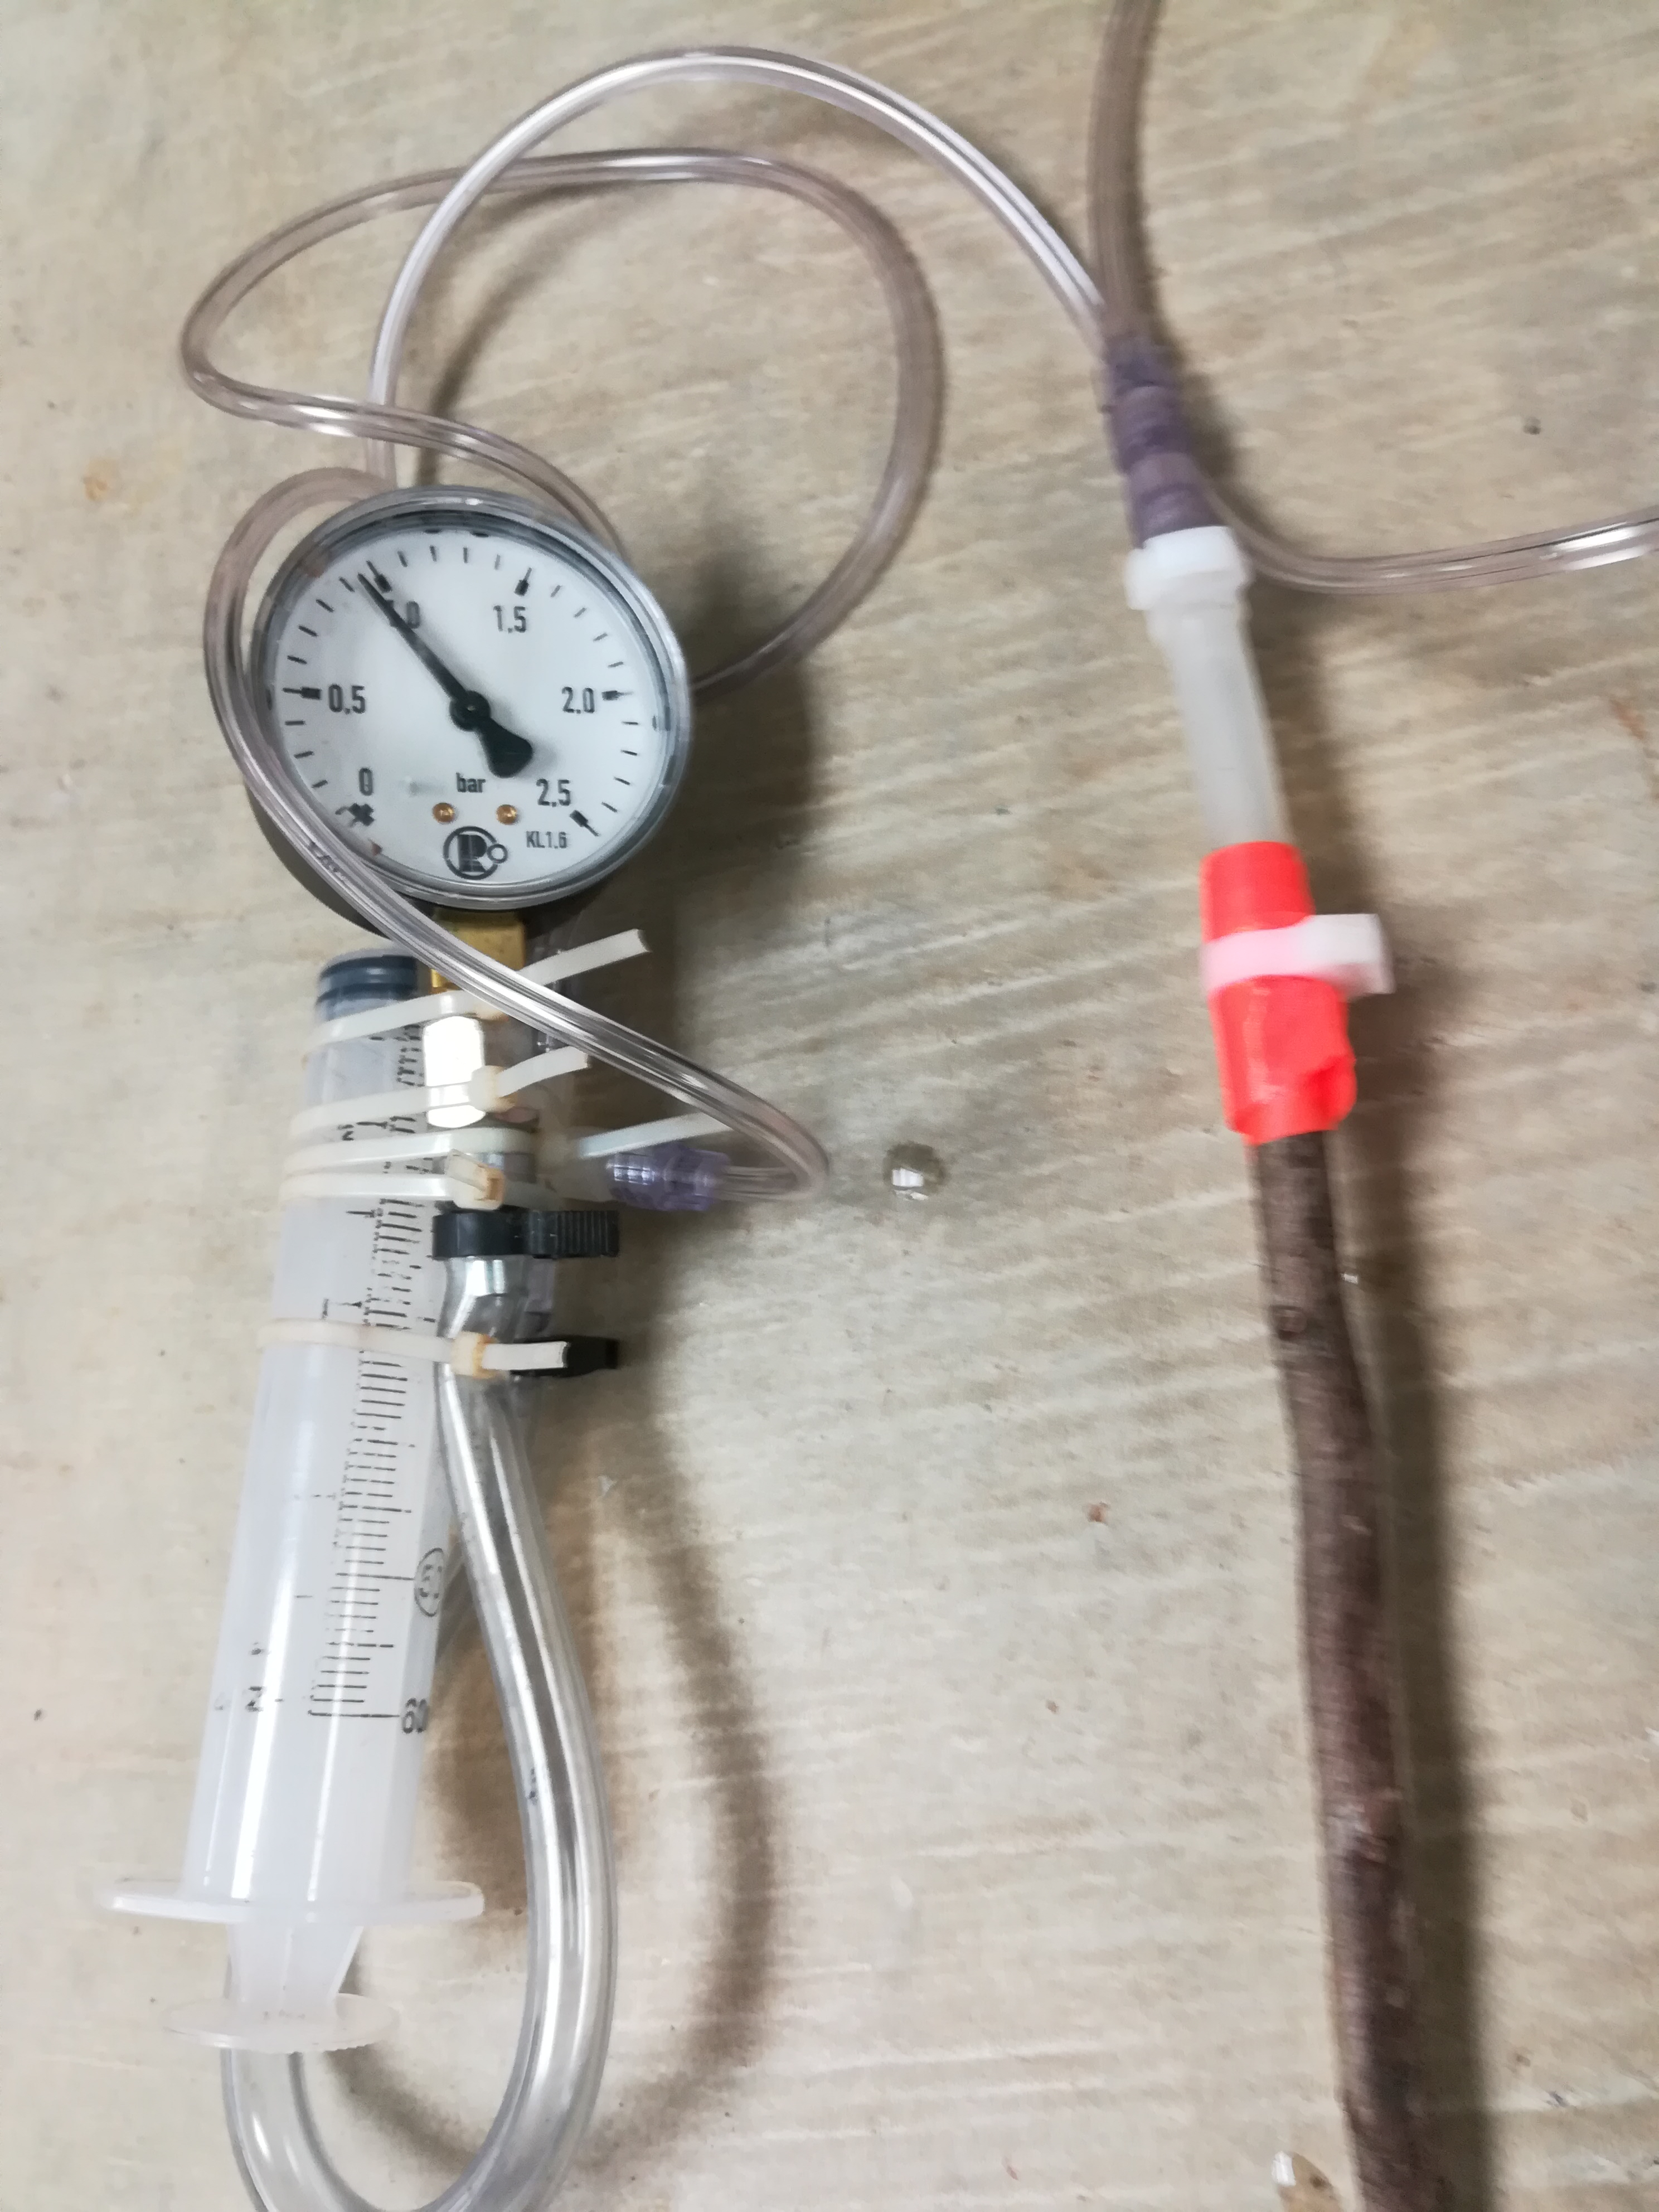
\includegraphics[width =\tw]{pictures/VL2.jpg}}
	
	    \only<3->{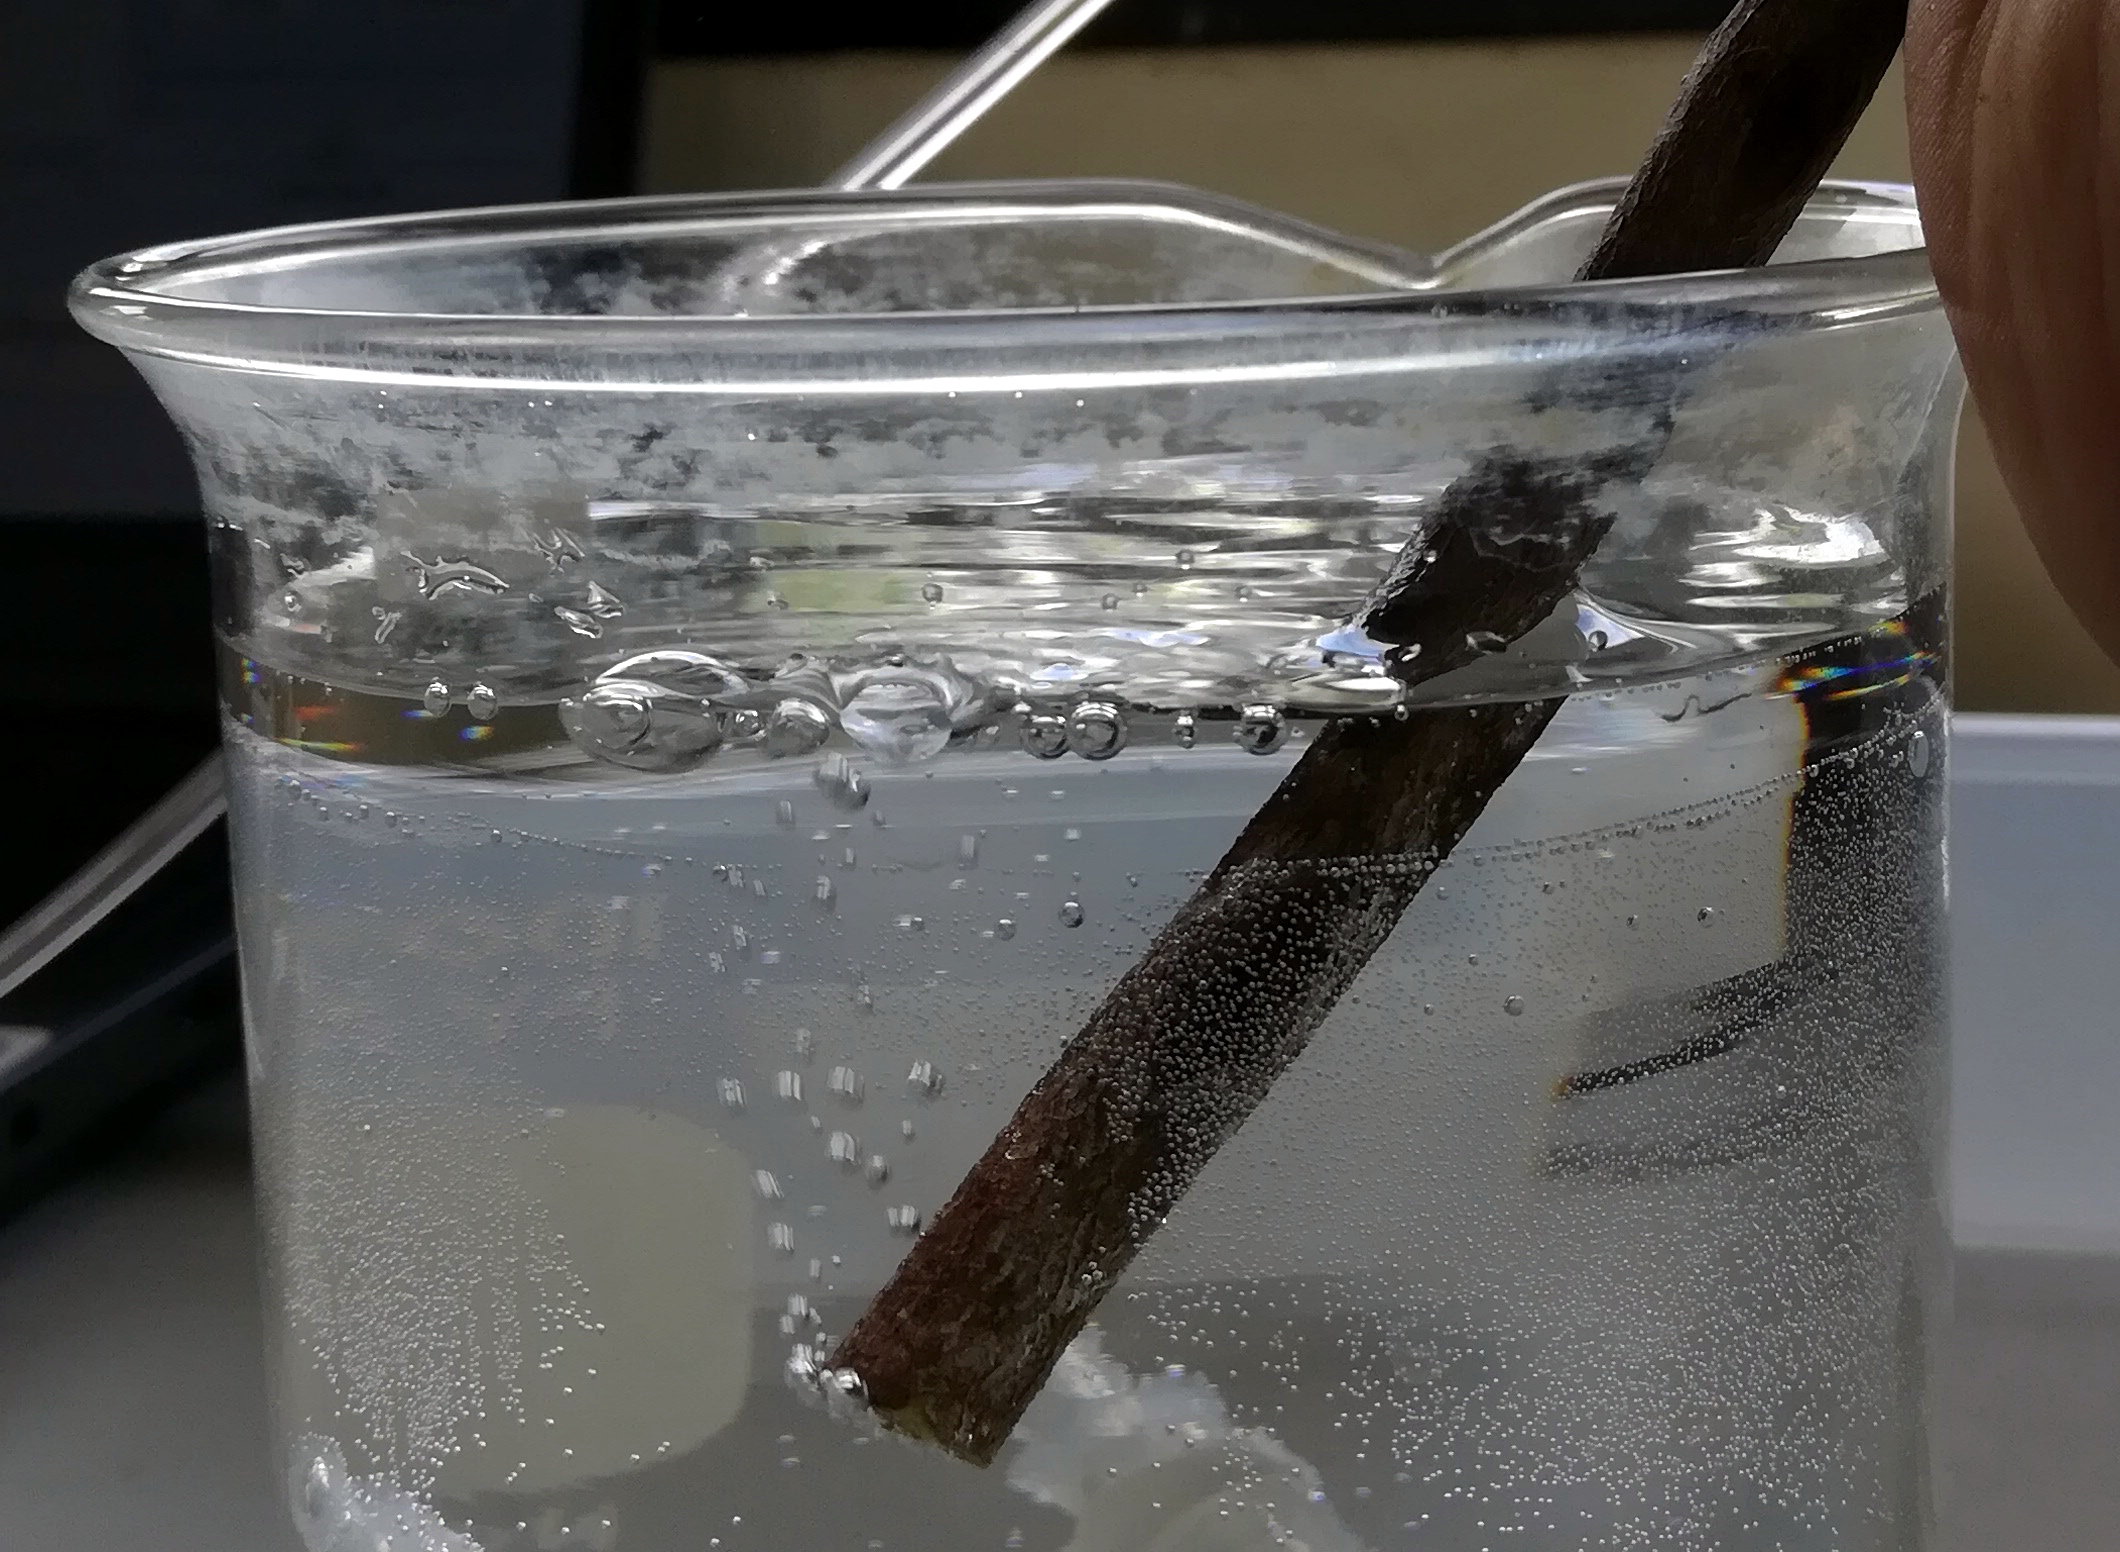
\includegraphics[width =\tw]{pictures/VL3.jpg}}	  
	\end{minipage}			
\end{frame}

\begin{frame}
	\frametitle{Conexión de las muestas}
	\begin{minipage}{.68\tw}
		\begin{itemize}
			\item<1- |alert@1> Conectar con tubo de látex y llenar con solución de medición
			\item<2- |alert@2> Conectar con conector multiple del XylEm plus
			\item<3- |alert@3> \textbf{Muy importante: ¡No debe haber ningunas burbujas de aire!}
	    \end{itemize}	    	
	\end{minipage}
	\begin{minipage}{0.3\tw}
		\only<1>{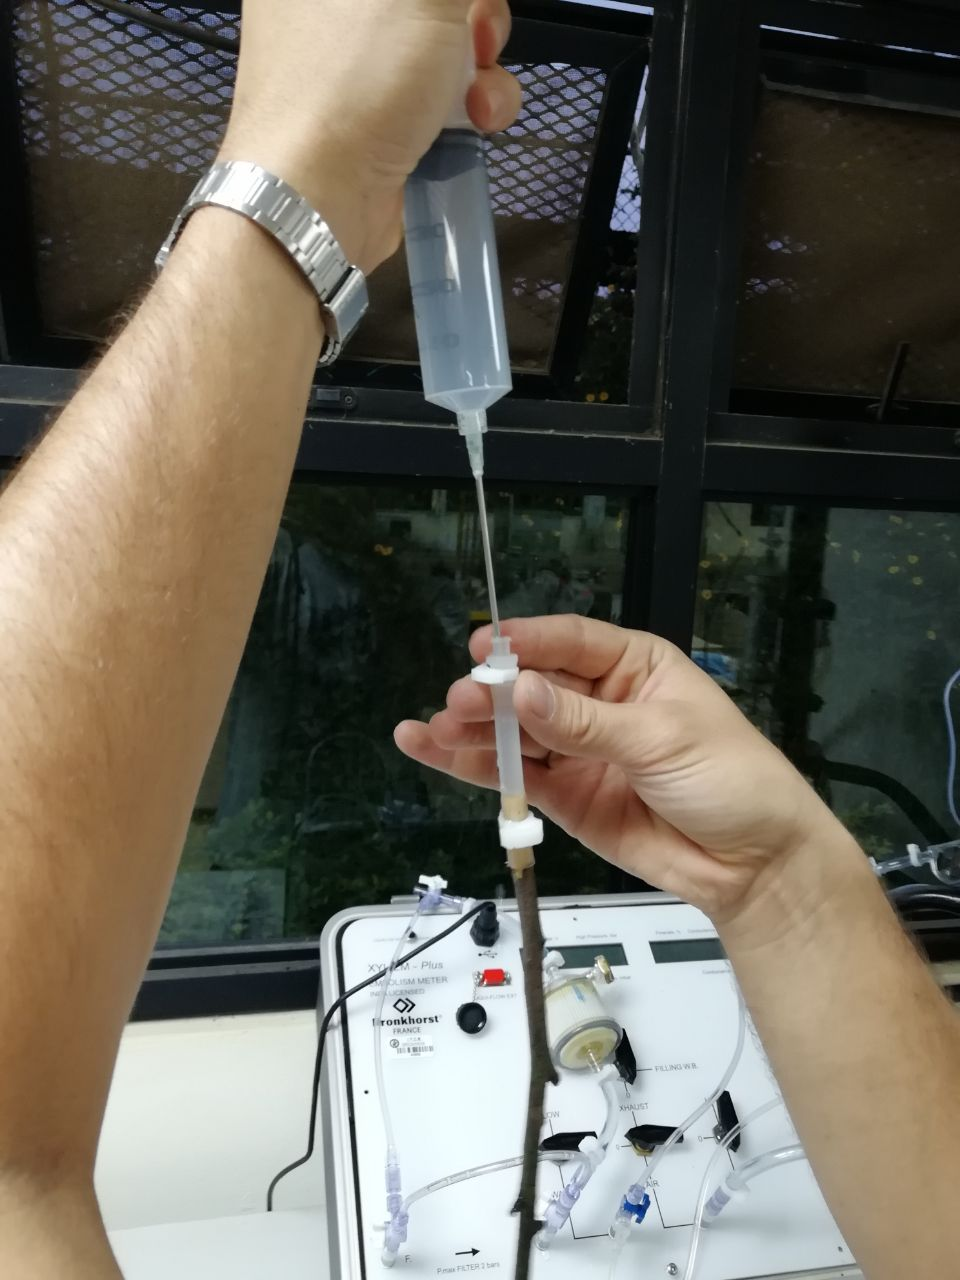
\includegraphics[width =\tw]{pictures/conectar.jpg}}
		
		\only<2>{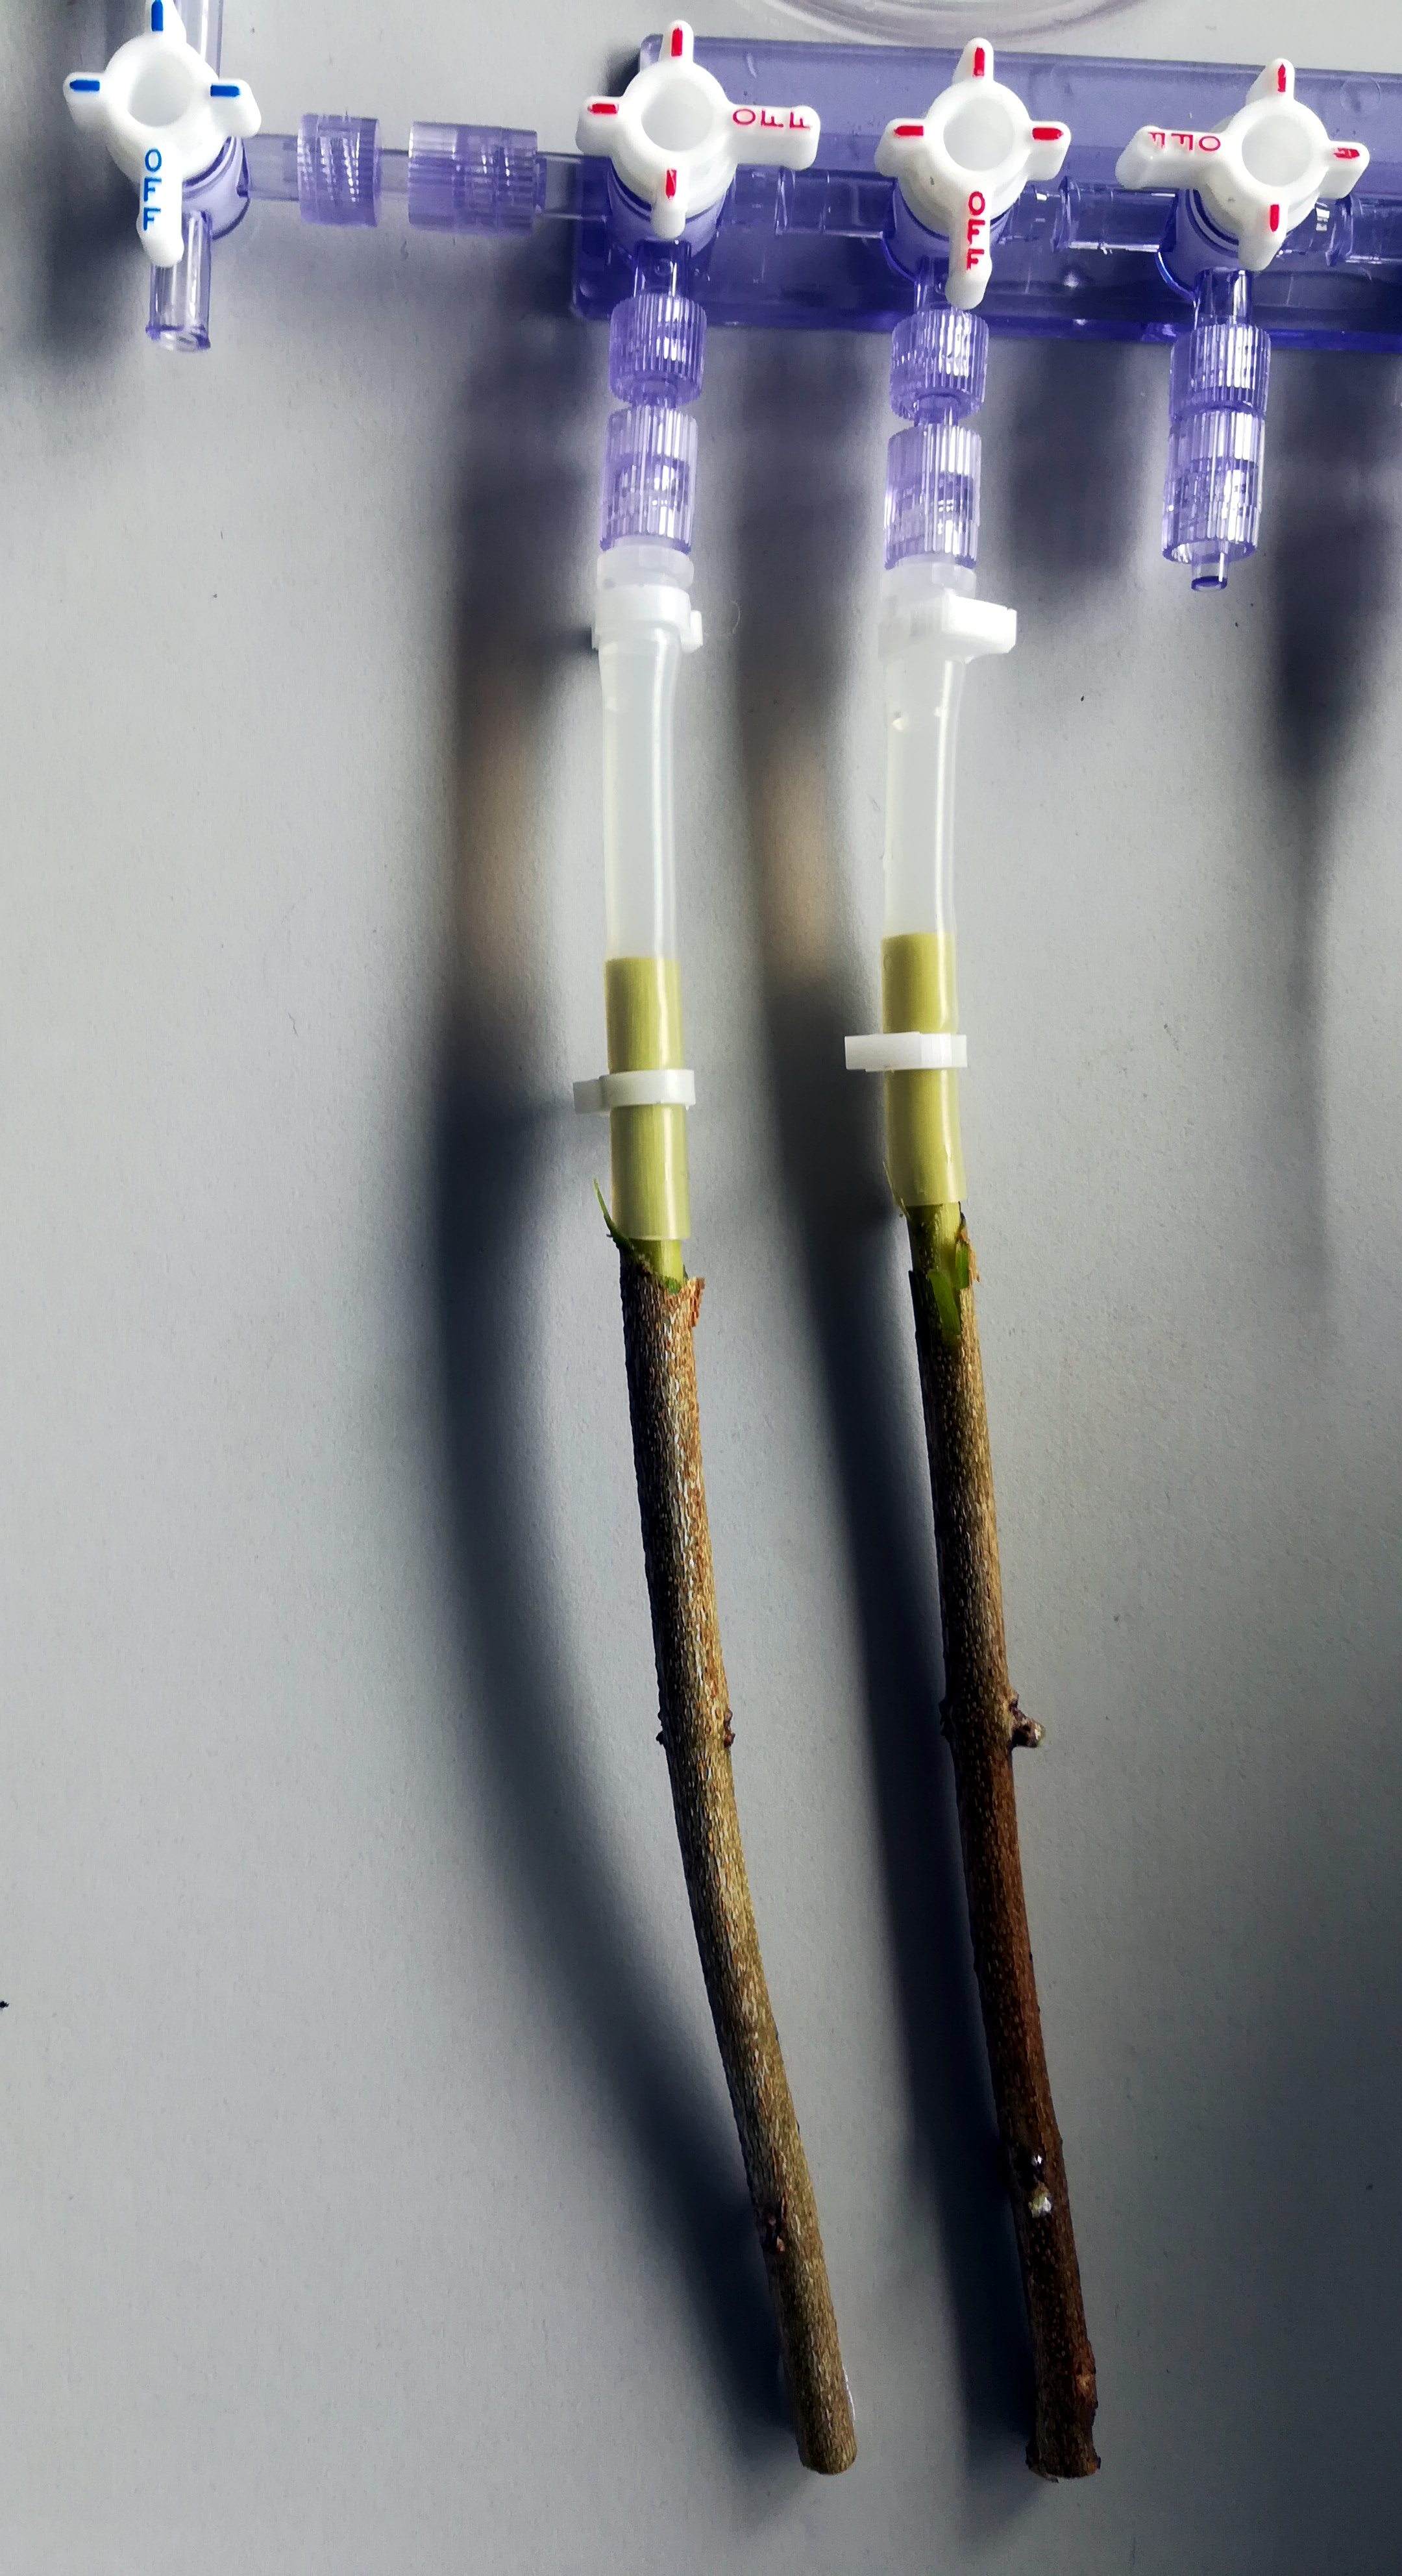
\includegraphics[width =\tw]{pictures/samples1.jpg}}	
		
    	\only<3>{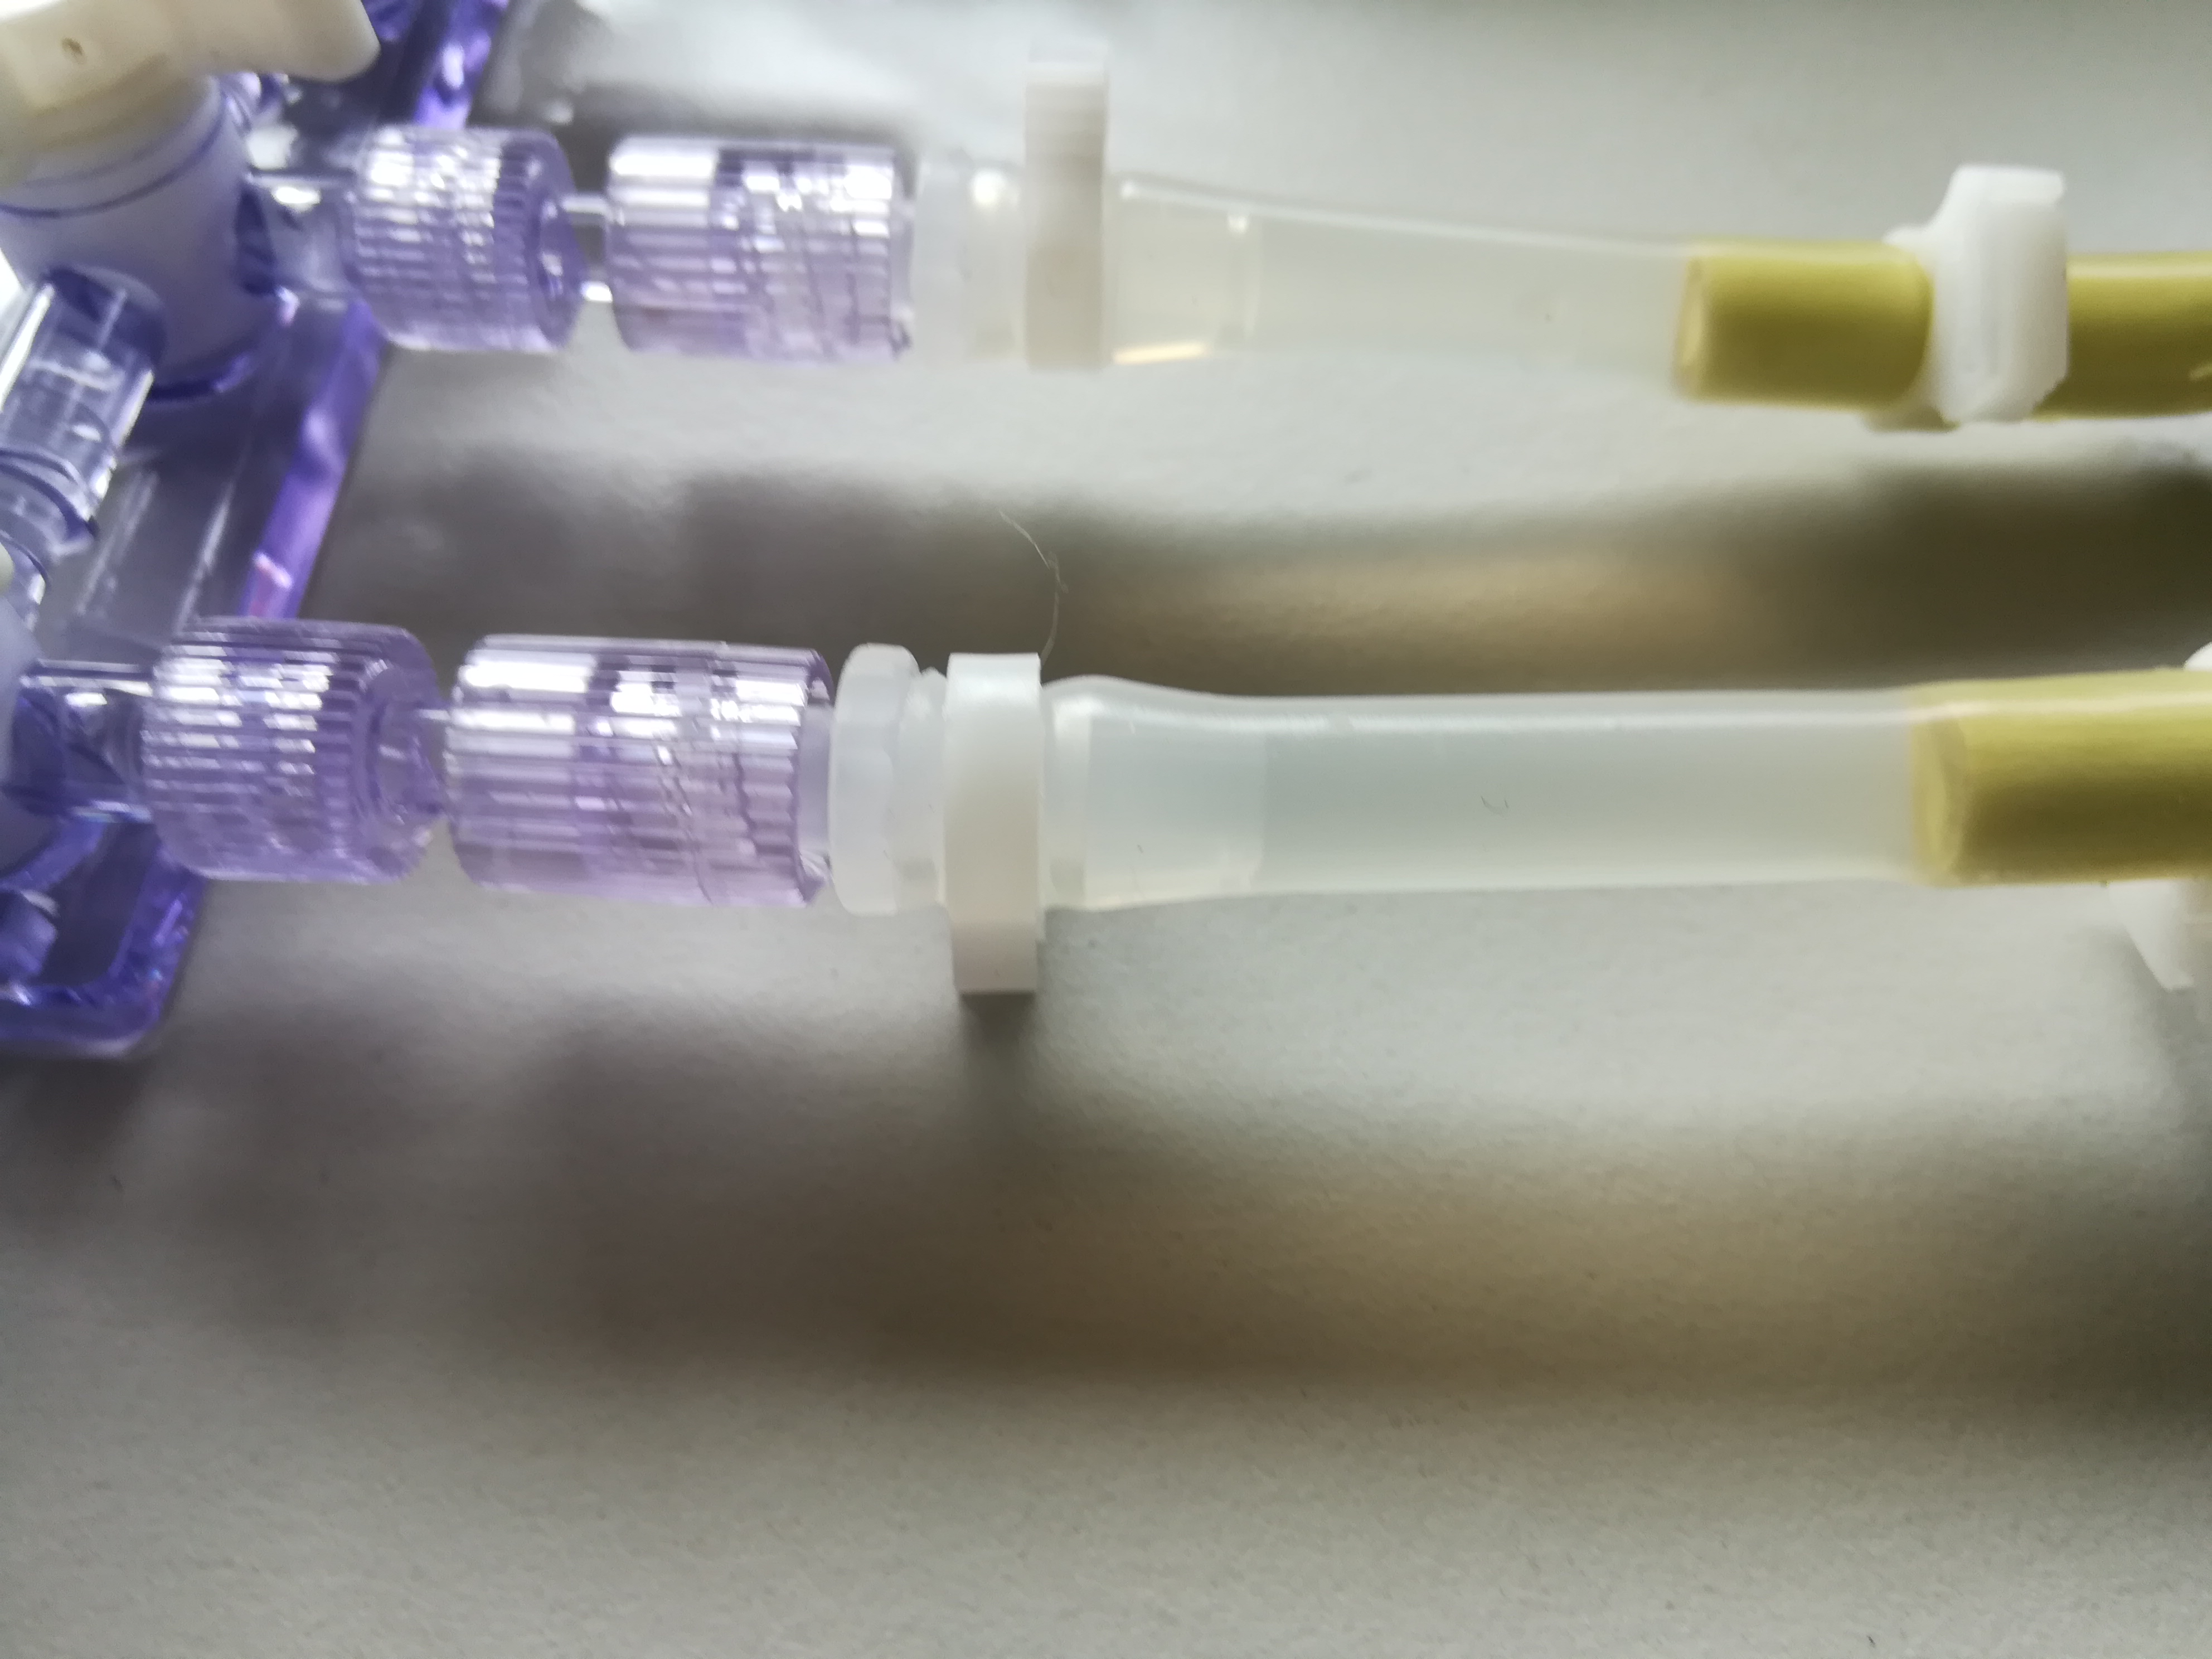
\includegraphics[width =\tw]{pictures/samples2.jpg}}				  
	\end{minipage}	
\end{frame}

\begin{frame}
	\frametitle{Proceso de medición} 
	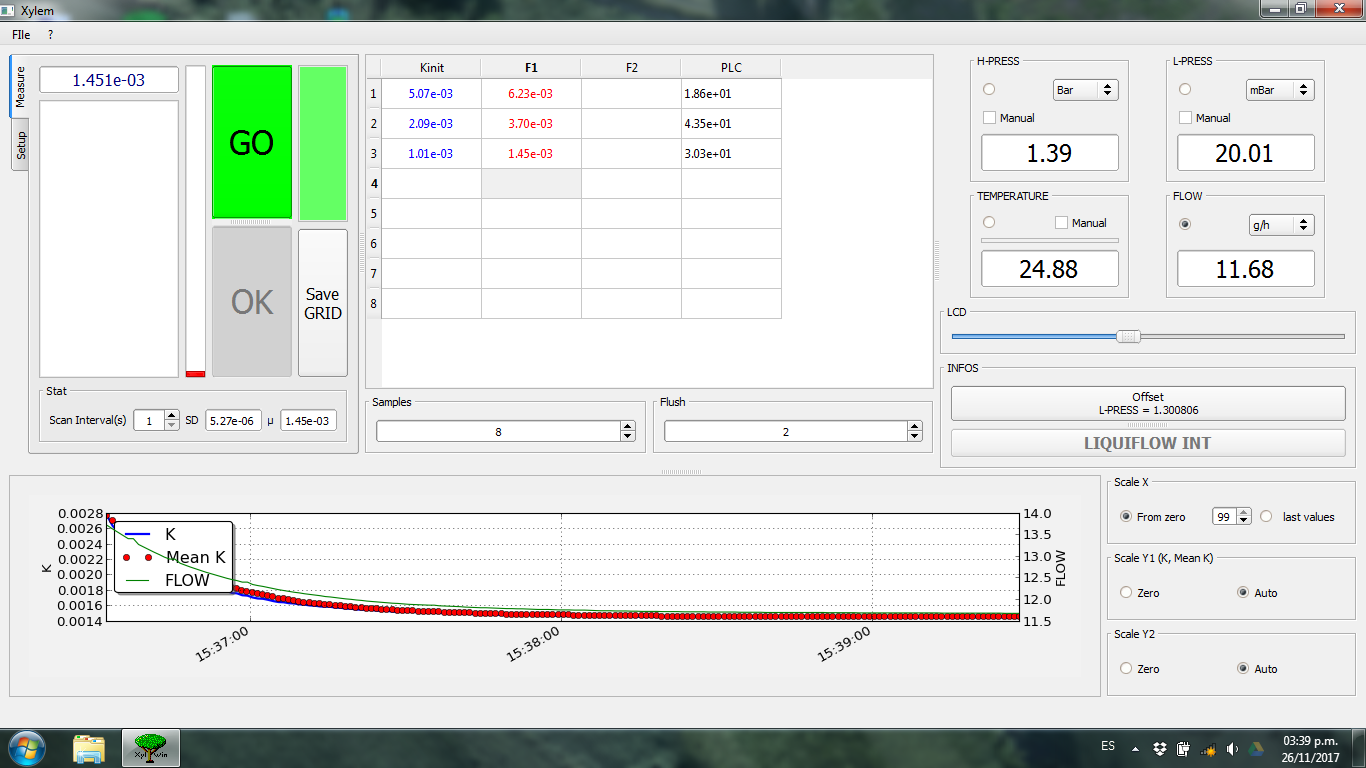
\includegraphics[width = \tw]{pictures/screenshot.png}
	\begin{itemize}[<+-| alert@+>]
		\item Proceso de medición automatizado por \textbf{XylWin software}
		\item Permite la medición paralela varias muestras 
	\end{itemize}	
\end{frame}


\begin{frame}
	\frametitle{Proceso de medición} 
	\textbf{Protocolo}
		\begin{itemize}[<+->]
			\item[\blue{1)}] Poner XylEm en \textit{low pressure mode} y medir primer muestra hasta que el XylWin software indica que la conductancia esté constante \alert<1>{(\Rar\ equilibrio dinámico)}
			\item[\blue{2)}] Repetir paso \Blue{1)}\ para las otras muestras conectadas
			\item[\blue{3)}] Poner XylEm en \textit{high pressure mode} y enjuagar muestras por 10 min
			\item[\blue{4)}]Repetir pasos \Blue{1)} y \Blue{2)}\ hasta que la conductancia no se cambia después de enjuagar las muestras
		\end{itemize}	
		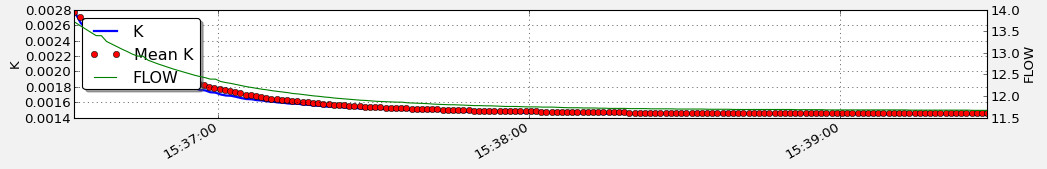
\includegraphics[width = \tw]{pictures/screenshot_detail.jpg}
\end{frame}


\begin{frame}
	\frametitle{Avisos prácticos para el uso del XylEm Plus}
	\begin{itemize}[<+- |alert@+>]
		\item Antes de cada día de medición, revisar que no haya ningunas burbujas de aire en los tubos y filtros del XylEm 	
		\item No usar solución de medición preparada hace más de 2-3 días	
		\item Muy importante: Corrección de \textit{pressure offset}
		\item Después de un tiempo más largo de desuso o cada 1-2 semanas: limpiar tubos (¡no filtros!) con solución de hipoclorito de sodio (50 ml de "lejía" por 2 l de agua)	
	\end{itemize}		
\end{frame}



%%%%%%%%%%%%%%%%%%%%%%%%%%%%%%%%%%%%%%%%%%%%%%%%%%%%%%%%%%%%%%%%%%%%
\section{Bomba de Scholander}
%%%%%%%%%%%%%%%%%%%%%%%%%%%%%%%%%%%%%%%%%%%%%%%%%%%%%%%%%%%%%%%%%%%%
\begin{frame}
		\frametitle{Bomba de Scholander}
		\centering{
		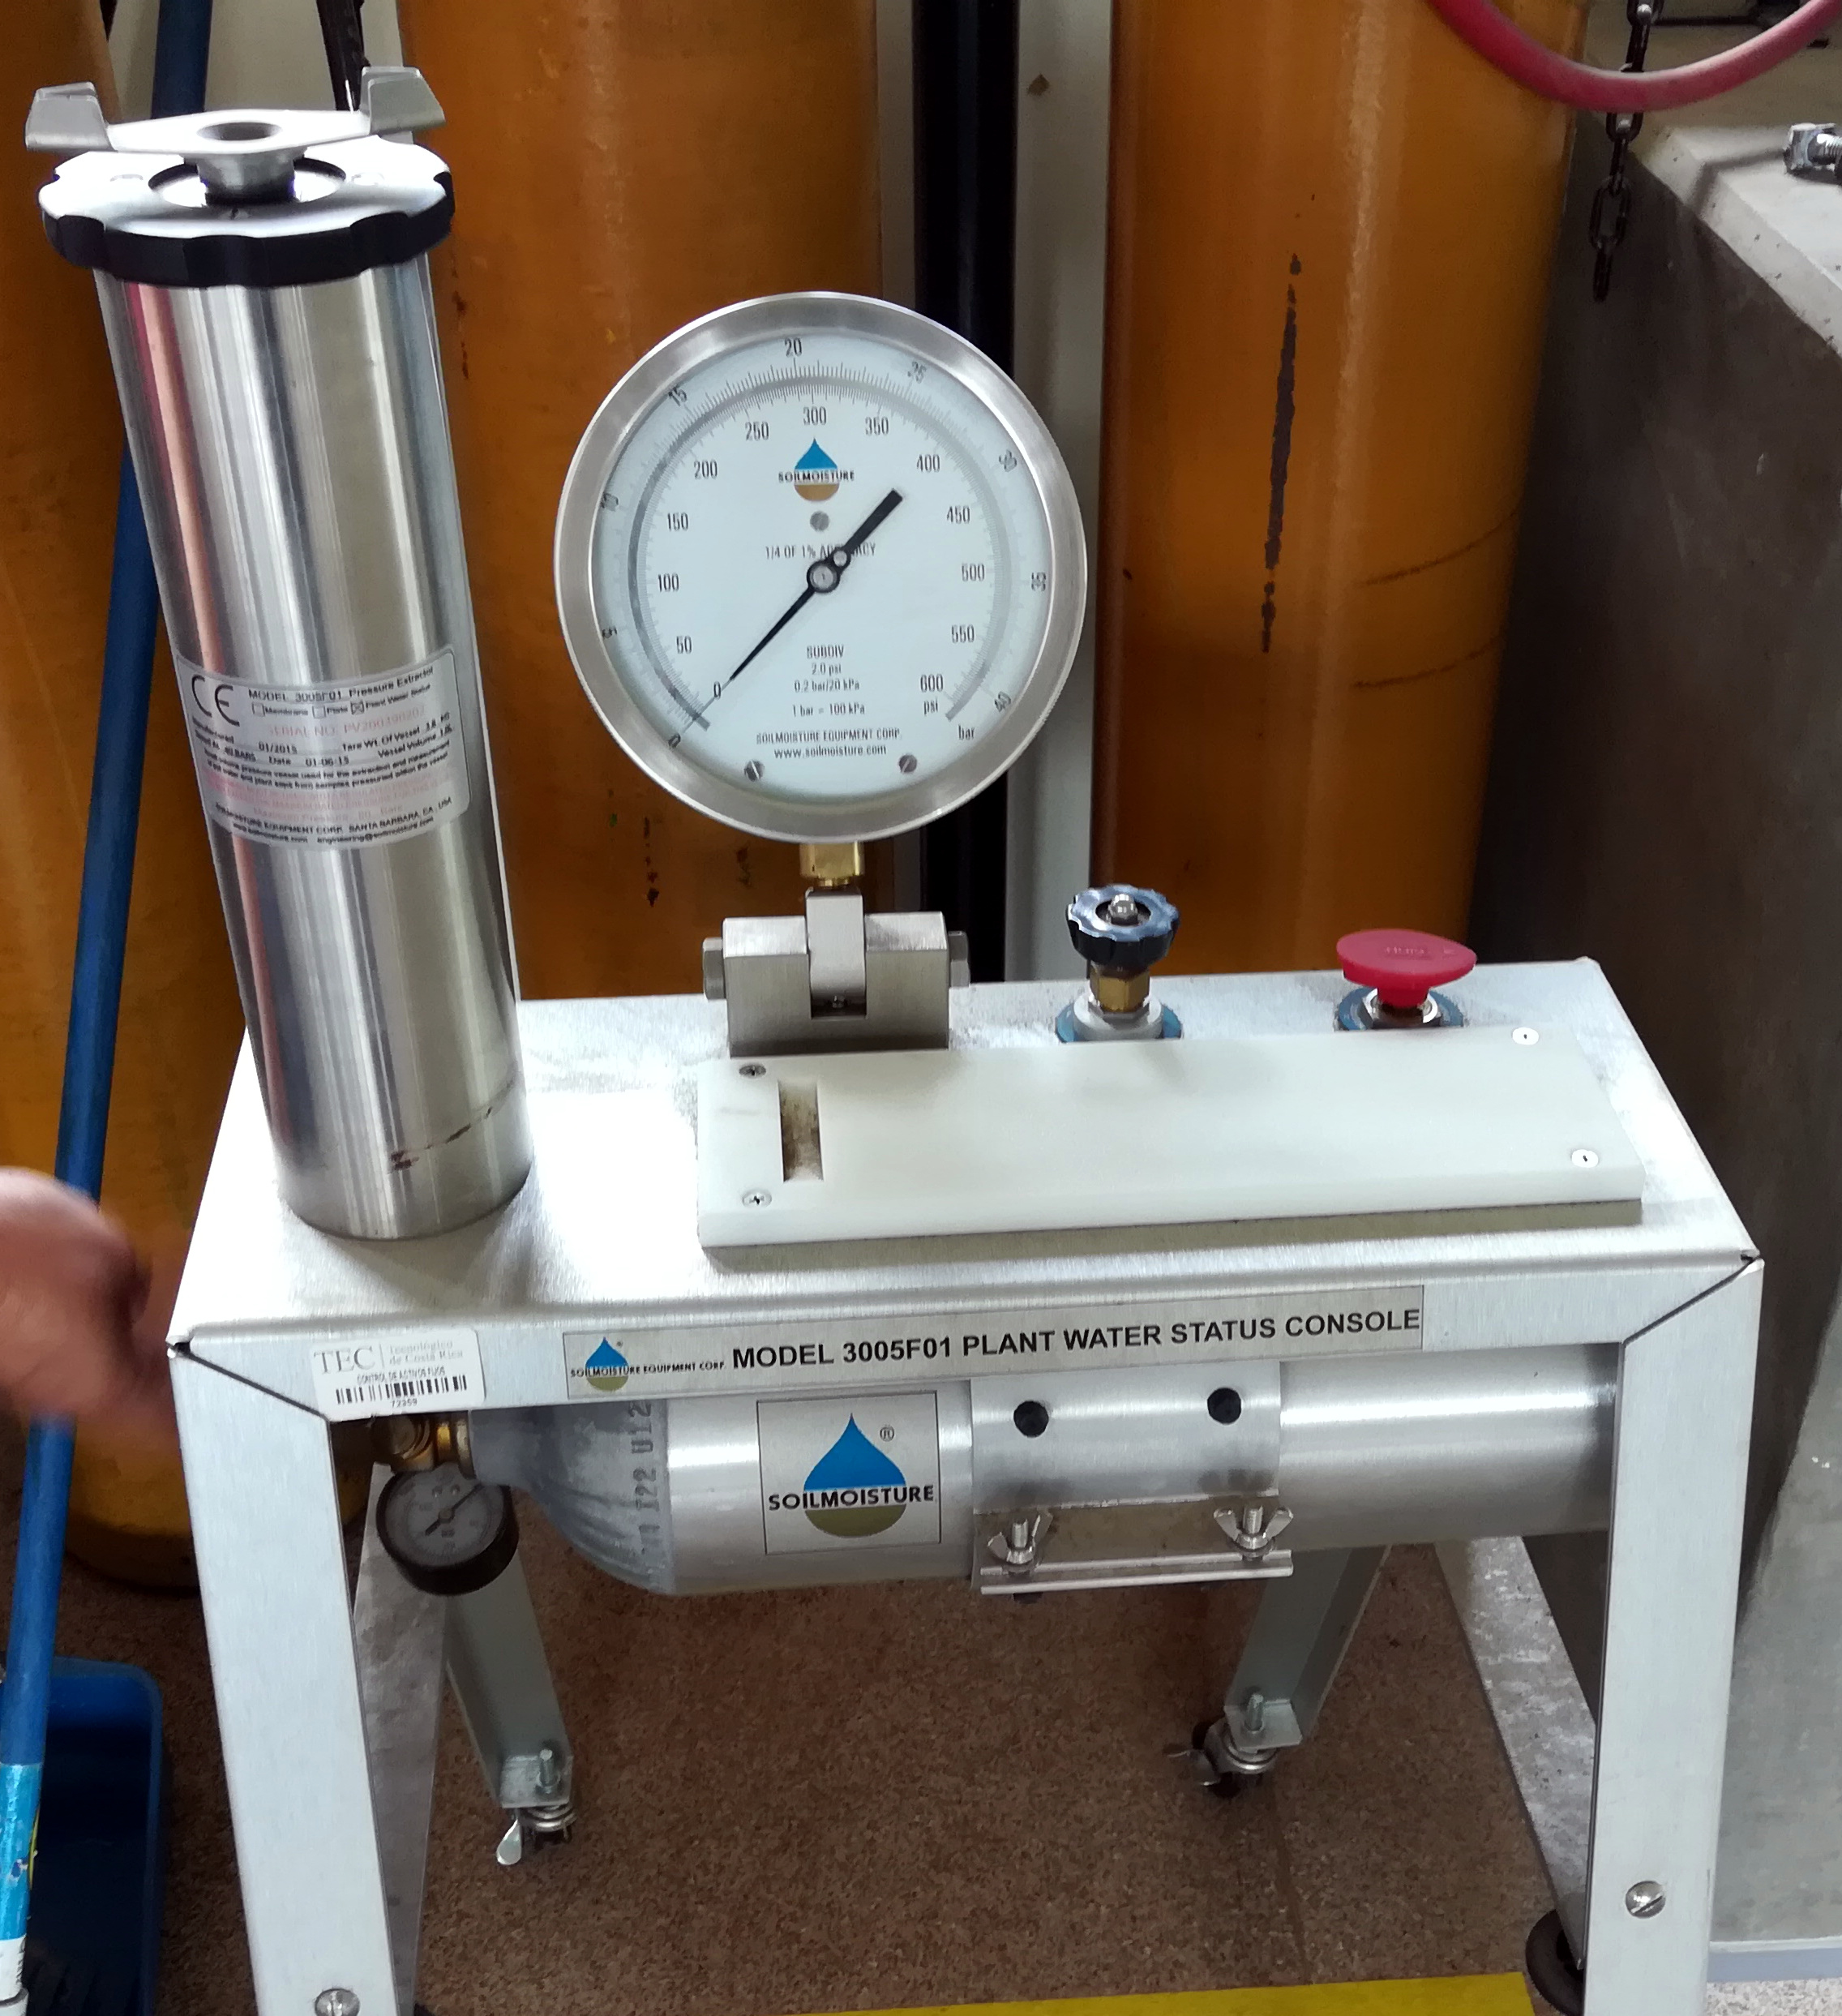
\includegraphics[width =0.35\tw]{pictures/bomba1.jpg}
		\quad	
		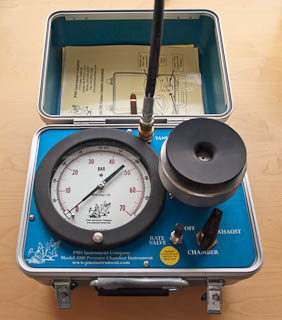
\includegraphics[width =0.35\tw]{pictures/bomba2.jpg}} 
 \begin{itemize}
 	\item Aparato para la medición del \alert{potenciál hídrico} de hojas o ramas
 	\item Método desarrollado por \alert{Scholander et al. (1965)}
 	\item Muy bien estudiado y establecido
 	\item Muchos modelos comerciales diferentes disponibles  \end{itemize}	    
\end{frame}

\begin{frame}
	\frametitle{Funcionamiento de la Bomba de Scholander}
	\centering{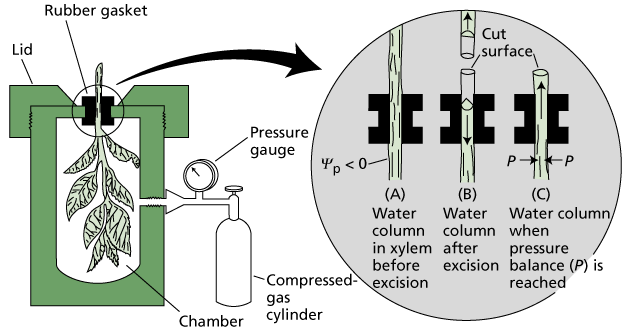
\includegraphics[width = 0.8\tw]{pictures/taiz_zeiger_2000.png}}
	
	\begin{itemize}
		\item<only@1> Muestra en el dentro de una cámara de presión
		\item<only@1> Presión se aumenta lentamente hasta que las primeras gotas de savia salgan del xylem 
		\item<only@2-> Cuando la savia llega a la superficie del corte: equilibrio entre presión interna de la hoja y presión externa del aire 
		\item<only@2-| visible@3>[\Rar] \textbf{\alert{Potencial hídrico} de la muestra}
	\end{itemize}
	
		\centering{\quelle{\textbf{Ilustración:} Taiz \& Zeiger, 2002.}}		
\end{frame}

\begin{frame}
	\frametitle{Protocolo de medición}
	\begin{itemize}[<+- |alert@+>]
		\item Cortar muestra con cuchilla afilada
		\item Colocar muestra en el tapón de la bomba de Scholander y cerrar la junta de goma firmemente
		\item Cerrar la cámara de presión (cuidado al no aplastar ningunas hojas)
		\item Aumentar presión lentamente con la válvula de aguja (no más que 3 bar/min) y observar la superficie del corte con una lupa
		\item Cuando agua empieza salir del corte, revisar la presión indicada por el manómetro 
	\end{itemize}		
\end{frame}

\begin{frame}
	\centering{	
	\begin{minipage}{0.6 \tw}
		\begin{block}{\textbf{Aviso importante}}
			\textbf{¡Nunca cerrar el empaque de aguja con fuerza, se daña facilmente!}
		\end{block}
		
		\vspace{1em}
		\visible<2>{
		\begin{alertblock}{\textbf{Aviso de Seguridad}}
			\textbf{¡Siempre usar gafas de seguridad!}}
		\end{alertblock}	
	\end{minipage}	
}
\end{frame}


%%%%%%%%%%%%%%%%%%%%%%%%%%%%%%%%%%%%%%%%%%%%%%%%%%%%%%%%%%%%%%%%%%%
\section{Referencias}
%%%%%%%%%%%%%%%%%%%%%%%%%%%%%%%%%%%%%%%%%%%%%%%%%%%%%%%%%%%%%%%%%%%%

\begin{frame}
	\frametitle{Prometheus Wiki}

\Blue{ \huge \url{http://prometheuswiki.org/}}

\vspace{0.5 em}
\begin{itemize}[<+-| alert@+>]
	\item Fuente de información muy recomendada para métodos de fisiología de plantas	
	\item Muchos métodos explicados al detalle por sus autores con muchas imágenes 
	\item Muchas veces más detallados que las publicaciones originales de los métodos
	\item Acceso libre y gratuito
\end{itemize}
\end{frame}

\begin{frame}
	\frametitle{Prometheus Wiki}
	\begin{changemargin}{-2em}{-2em}
		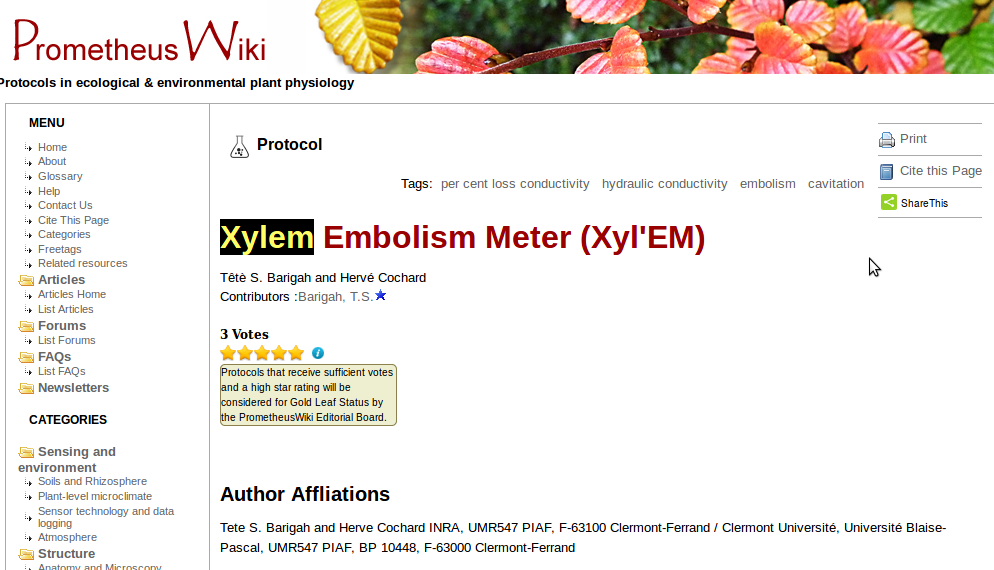
\includegraphics[width = \paperwidth]{pictures/prometheus.png}
	\end{changemargin}
\end{frame}




\begin{frame}%[allowframebreaks]
\frametitle{Lista de referencias}\label{bib}
\color{black}
\begin{changemargin}{-1.5em}{-1.5em}
 {\footnotesize \justifying
\begin{itemize}
 
 \item \textbf{Cochard, H. (2002).} \textit{Xylem embolism and drought-induced stomatal closure in maize.} Planta, 215(3), 466-471.
 \item  \textbf{Cochard, H. (2013).} \textit{XYL’EM- Plus instruction manual and tutorial for xylem embolism measurements Version 2.1.} URL \url{https://www.bronkhorst.fr/fr/produits/xylem_embolie-metre/}
 \item \textbf{ Cochard, H. et al. (2000).} \textit{Cryo-scanning electron microscopy observations of vessel content during transpiration in walnut petioles. Facts or artifacts?} Plant Physiology, 124(3), 1191-1202.
 \item\textbf{ Cochard, H. et al. (2002).} \textit{Unraveling the effects of plant hydraulics on stomatal closure during water stress in walnut.} Plant Physiology, 128(1), 282-290. 
 \item \textbf{ Scholander, P. F. et al. (1965).} \textit{Sap pressure in vascular plants: negative hydrostatic pressure can be measured in plants.} Science, 148(3668), 339-346.
 \item \textbf{ Sperry, J. S. et al. (1988).} \textit{A method for measuring hydraulic conductivity and embolism in xylem.} Plant, Cell \& Environment, 11(1), 35-40.
 \item \textbf{Taiz, L., \& Zeiger, E. (2002).} \textit{Plant Physiology,} Sinauer Associates.
\end{itemize}
} 
\end{changemargin}
\end{frame}
\end{document}
